% Adaptive Dynamic Query Routing for Urdu Information Retrieval
% Formatted using the PLOS LaTeX template (plos_latex_template.tex, Version 3.8 Apr 2026)
%
% NOTE ON FIGURES: PLOS submissions normally require figures to be uploaded as
% SEPARATE files rather than embedded in the manuscript LaTeX. The \includegraphics
% calls below are kept in place so the document compiles into a complete, readable
% PDF; remove/externalize them at final submission time per PLOS figure guidelines
% (https://journals.plos.org/plosone/s/figures).

\documentclass[10pt,letterpaper]{article}
\usepackage[top=0.85in,left=1in,right=1in,footskip=0.75in]{geometry}

% amsmath and amssymb packages, useful for mathematical formulas and symbols
\usepackage{amsmath,amssymb}

% Use adjustwidth environment to exceed column width (see example table in text)
\usepackage{changepage}

% textcomp package and marvosym package for additional characters
\usepackage{textcomp,marvosym}

% cite package, to clean up citations in the main text. Do not remove.
\usepackage{cite}

% Use nameref to cite supporting information files (see Supporting Information section for more info)
\usepackage{nameref,hyperref}

% line numbers
\usepackage[right]{lineno}

% ligatures disabled
\usepackage[nopatch=eqnum]{microtype}
\DisableLigatures[f]{encoding = *, family = * }

% color can be used to apply background shading to table cells only
\usepackage[table]{xcolor}

% array package and thick rules for tables
\usepackage{array}

% create "+" rule type for thick vertical lines
\newcolumntype{+}{!{\vrule width 2pt}}

% create \thickcline for thick horizontal lines of variable length
\newlength\savedwidth
\newcommand\thickcline[1]{%
  \noalign{\global\savedwidth\arrayrulewidth\global\arrayrulewidth 2pt}%
  \cline{#1}%
  \noalign{\vskip\arrayrulewidth}%
  \noalign{\global\arrayrulewidth\savedwidth}%
}

% \thickhline command for thick horizontal lines that span the table
\newcommand\thickhline{\noalign{\global\savedwidth\arrayrulewidth\global\arrayrulewidth 2pt}%
\hline
\noalign{\global\arrayrulewidth\savedwidth}}

% Text layout
\raggedright
\setlength{\parindent}{0.5cm}
\textwidth 5.25in
\textheight 8.75in

% Bold the 'Figure #' in the caption and separate it from the title/caption with a period
% Captions will be left justified
\usepackage[aboveskip=1pt,labelfont=bf,labelsep=period,justification=raggedright,singlelinecheck=off]{caption}
\renewcommand{\figurename}{Fig}

% Please use the included `plos2025.bst` as your BibTeX style
\bibliographystyle{plos2025}

% Remove brackets from numbering in List of References
\makeatletter
\renewcommand{\@biblabel}[1]{\quad#1.}
\makeatother

% ---- Additional packages required by this manuscript's content (tables, figures, equations) ----
\usepackage{booktabs}
\usepackage{multirow}
\usepackage{graphicx}
\usepackage{rotating}
\usepackage{float}
\usepackage{tikz}
\usepackage{pgfplots}
\pgfplotsset{compat=1.18}
\usetikzlibrary{shapes.geometric,arrows.meta,positioning,fit}

% Header and Footer with logo
\usepackage{lastpage,fancyhdr}
\usepackage{epstopdf}
\pagestyle{fancy}
\fancyhf{}
\rfoot{\thepage/\pageref{LastPage}}
\renewcommand{\headrulewidth}{0pt}
\renewcommand{\footrule}{\hrule height 2pt \vspace{2mm}}
\fancyheadoffset[L]{2.25in}
\fancyfootoffset[L]{2.25in}
\lfoot{\today}

%% Include all user-defined macros below

%% END MACROS SECTION


\begin{document}
\vspace*{0.2in}

% Title must be 250 characters or less.
\begin{flushleft}
{\Large
\textbf{Adaptive dynamic query routing for Urdu information retrieval}
}
\newline
% Insert author names, affiliations and corresponding author email (do not include titles, positions, or degrees).
\\
Hashim Shazad\textsuperscript{1*},
Adnan Aslam\textsuperscript{1}
\\
\bigskip
\textbf{1} Department of Creative Technologies, Air University, Islamabad, Pakistan
\\
\bigskip

% Use the asterisk to denote corresponding authorship and provide email address in note below.
* abbasihashim30@gmail.com

\end{flushleft}

\section*{Abstract}
Urdu search mixes native script with Roman Urdu. ULTRA still routes queries with one cutoff: 150 characters. A short question can need the article. A long question can be asking for a fact that already sits in a headline.

We keep SHORT and LONG but change the meaning. SHORT means a headline is probably enough. LONG means the user likely needs the body. An eight-feature SVM makes the call. Headlines and full articles live in two indexes. Confidence is a light: high searches one index, medium mixes both, low expands then mixes. The Roman Urdu word list on disk has 198 pairs (older drafts said 179).

Three tests are kept apart. On 50 frozen Phase~3B queries the SVM hit 86\% and a six-word rule hit 84\% (McNemar $p=1.0$). On 40 trap queries the SVM reached 60\%, word count 20\%, and $\theta=150$ 50\% (McNemar 16--0). That trap gain is almost entirely in 18 queries with why/how/fact wording; on the other 22 both systems score 27.27\%. Four hundred graded judgments on the same 40 queries do not reward the SVM at P@5 (word count 36.50\%, always-headline and $\theta=150$ 35.00\%, always-full 34.25\%, SVM 33.00\%). nDCG@5 is highest for always-headline (0.6868).

The character cutoff is a weak proxy for need. The SVM helps when the wording carries an obvious cue. On this news collection it does not improve early precision. We report that gap as part of the study.
\clearpage
\newgeometry{top=0.85in,left=1in,right=1in,footskip=0.75in}
\linenumbers

% ============================================================
\section*{Introduction}
% ============================================================

\subsection*{Background}

Urdu is spoken by over 230 million people worldwide and serves as the national language of Pakistan and one of the officially recognized languages of India, yet it remains substantially underserved within contemporary information retrieval (IR) research \cite{daud2017urdu}. Unlike high-resource languages such as English, where dense retrieval, neural ranking, and large language model (LLM)-based query understanding have matured rapidly -- driven by pretrained transformer encoders \cite{devlin2019bert} and dense dual-encoder retrievers \cite{karpukhin2020dpr} -- Urdu IR continues to face persistent challenges rooted in script complexity, morphological richness, and the informal, code-mixed nature of user-generated queries \cite{daud2017urdu, kazi2025urdu}. A particularly acute challenge is the widespread use of Roman Urdu -- Urdu written using the Latin script -- in everyday digital communication and search queries, which introduces significant lexical and orthographic variation that conventional retrieval pipelines are not designed to handle \cite{hussain2025qlora}.

The scarcity of standardized evaluation resources compounds this problem. Early efforts such as the Collection for Urdu Retrieval Evaluation (CURE) \cite{iqbal2021cure} and, more recently, the translated Urdu MS MARCO baseline \cite{butt2024urdumsmarco}, have begun to establish benchmarks for Urdu IR, but adaptive, query-aware retrieval strategies for Urdu remain largely unexplored.

The ULTRA framework, proposed by Bashir, Qaiser, and Hussain \cite{bashir2026ultra}, represents a recent effort in this direction, introducing a dual-embedding, query-length-sensitive routing scheme that distinguishes between short, intent-oriented queries and longer, context-rich queries using a threshold-based decision process. However, ULTRA's routing mechanism relies on a \emph{static} query-length threshold, which does not adapt to the full range of linguistic characteristics a real Urdu query may exhibit -- including lexical diversity, Roman Urdu transliteration, and question structure. This mirrors a broader challenge identified in the general IR literature: Arabzadeh et al.\ \cite{arabzadeh2021predicting} showed that a learned classifier for routing queries between sparse and dense retrieval strategies can substantially outperform static rules, though their work was developed and evaluated only for English.

This paper extends the ULTRA framework by replacing its static, length-based routing threshold with an adaptive, dynamic query routing mechanism. The proposed system classifies incoming Urdu (and Roman Urdu) queries using a lightweight, eight-feature Support Vector Machine (SVM) classifier and routes them to the most appropriate retrieval configuration in real time, combined with a confidence-based tiered escalation strategy for ambiguous queries.

\subsection*{Problem statement}

Existing Urdu information retrieval systems, including the ULTRA framework on which this paper builds, predominantly employ static, threshold-based routing that applies a fixed decision rule regardless of the deeper linguistic characteristics of a query -- such as lexical diversity, script type (native Urdu vs.\ Roman Urdu), or the presence of interrogative structure. This static approach results in suboptimal retrieval performance for queries that deviate from the assumption the threshold was tuned for, particularly Roman Urdu queries, which suffer from inconsistent transliteration and vocabulary sparsity \cite{hussain2025qlora}. Preliminary evaluation of static threshold-based routing on a diverse Urdu query set shows accuracy as low as 50\%, representing a critical reliability gap for real-world deployment.

\subsection*{Research questions}

\textbf{RQ1:} Can query-level structural and linguistic features (e.g., character length, lexical diversity, Urdu character ratio, presence of question words) reliably predict the optimal retrieval configuration for a given Urdu query?

\textbf{RQ2:} Does a dynamic, machine learning-based query routing mechanism significantly outperform static threshold-based routing, of the kind used in the base ULTRA framework \cite{bashir2026ultra}, on frozen need labels, and does that classification gain show up as P@5 when SHORT and LONG open two different indexes?

\textbf{RQ3:} Can a confidence-based tiered routing strategy further improve system reliability and efficiency by selectively escalating low-confidence queries to more computationally intensive retrieval methods while resolving high-confidence queries through a lightweight classifier?

\subsection*{Objectives}

\begin{itemize}
    \item \textbf{Dynamic query classification:} Design and train a dynamic SVM-based classifier that predicts optimal query routing decisions using eight structural and linguistic features extracted from Urdu and Roman Urdu queries.
    \item \textbf{Roman Urdu support:} Develop and expand a Roman Urdu transliteration dictionary (198 pairs on disk; older drafts said 179) to cover Roman Urdu queries.
    \item \textbf{Confidence-based tiered routing:} Implement a three-tier confidence routing mechanism balancing retrieval accuracy with computational efficiency.
    \item \textbf{Comparative evaluation:} Benchmark the proposed dynamic routing approach against static threshold-based routing and commercial LLM-based routing methods on frozen Phase 3B, trap classification, and dual-index P@5, without mixing development 100\% into those tables.
    \item \textbf{Robustness validation:} Statistically validate the significance and generalizability of performance improvements through effect size analysis, learning curve evaluation, and validation on unseen queries.
\end{itemize}

\subsection*{Contributions}

\begin{enumerate}
    \item A restatement of SHORT/LONG as \emph{headline enough} vs.\ \emph{need the article}, not character length.
    \item Two retrieval indexes (headline vs.\ full article) plus HIGH/MEDIUM/LOW mixing on SVM confidence.
    \item Frozen Phase~3B: V2 SVM 86\% vs.\ word count 84\% (McNemar $p=1.0$).
    \item Frozen traps H001--H040: SVM 60\% vs.\ word count 20\% vs.\ $\theta=150$ 50\%, with a cue split that shows where the gain lives.
    \item Frozen dual-index P@5 on the same 40 queries: the classification win does not transfer (SVM 33.00\% vs.\ word count 36.50\%).
    \item A Roman Urdu dictionary of 198 pairs on disk, and an explicit refusal to quote development 100\% or 96\% as generalization.
\end{enumerate}

% ============================================================
\section*{Related work}
% ============================================================

Urdu information retrieval sits at the intersection of three research threads that are individually well studied for high-resource languages but remain fragmented for Urdu: general Urdu natural language processing, information retrieval benchmarking, and query-adaptive routing. This section reviews representative work in each thread and identifies the specific gap this paper addresses.

\subsection*{Urdu natural language processing}

Daud et al.\ \cite{daud2017urdu} conducted a comprehensive survey of Urdu language processing, cataloguing the linguistic characteristics that complicate computational treatment of the language: a cursive, context-sensitive Perso-Arabic script written right-to-left, rich morphology, and the absence of large-scale standardized corpora compared to English or Arabic. Their survey remains a foundational reference for understanding why Urdu NLP tools lag behind those available for high-resource languages.
\textbf{Research gap:} The survey catalogues foundational challenges but predates the transformer era and therefore does not address embedding-based retrieval or query-adaptive systems.
\textbf{Advantages:} Comprehensive coverage of Urdu-specific linguistic obstacles; widely cited foundational reference.
\textbf{Disadvantages:} No treatment of neural retrieval, query routing, or Roman Urdu-specific processing.

Kazi and Khoja \cite{kazi2025urdu} more recently proposed a framework for Urdu language document retrieval, applying deep learning techniques and evaluating the effect of different word embeddings on retrieval-adjacent tasks such as named entity recognition.
\textbf{Research gap:} The framework focuses on document-level representation quality rather than on how individual queries should be routed to different retrieval strategies based on their structural characteristics.
\textbf{Advantages:} Recent, transformer-era treatment of Urdu retrieval; empirically evaluates multiple embedding configurations.
\textbf{Disadvantages:} Does not address query-level adaptivity or Roman Urdu queries specifically.

\subsection*{Roman Urdu processing challenges}

Roman Urdu -- Urdu transliterated into the Latin script -- lacks a standardized spelling convention, meaning the same word may be written in multiple ways depending on the writer's phonetic intuition. Hussain et al.\ \cite{hussain2025qlora} addressed a related problem, fine-tuning large language models via QLoRA for offensive language detection in Roman Urdu-English code-mixed text, and explicitly identified inconsistent spelling, unstated grammar, and scarcity of labeled data as core obstacles for any Roman Urdu NLP task.
\textbf{Research gap:} Their work targets classification (offensive vs.\ non-offensive) rather than retrieval, and does not address how Roman Urdu queries should be routed differently from native-script Urdu queries within an IR pipeline.
\textbf{Advantages:} Demonstrates that parameter-efficient fine-tuning (QLoRA) can meaningfully improve Roman Urdu-English task performance despite data scarcity.
\textbf{Disadvantages:} Single-task focus (offensive language detection); does not generalize to query routing or retrieval precision.

More broadly, Sitaram et al.\ \cite{sitaram2019codeswitch} surveyed code-switched speech and language processing, characterizing the alternation between languages and scripts -- of which Roman Urdu is a script-level instance -- as a communicative phenomenon that conventional monolingual NLP pipelines are not designed to handle. Within Urdu specifically, Mehmood et al.\ \cite{mehmood2020xtreme} tackled the closely related task of Roman Urdu sentiment analysis, proposing a hybrid multi-channel architecture over custom Word2Vec, FastText, and GloVe embeddings and reporting F1-score gains of up to 9\% over adapted machine-learning baselines.
\textbf{Research gap:} Both works confirm that Roman Urdu requires script-aware, dedicated processing rather than being treated as a minor variant of native-script Urdu, but neither addresses query routing or retrieval: the code-switching survey is a general characterization of the problem space, and the sentiment hybrid targets classification rather than document retrieval.
\textbf{Advantages:} The survey provides a broad taxonomy of code-switching challenges applicable beyond Urdu; the sentiment hybrid empirically demonstrates that Roman Urdu-specific embeddings outperform generic ones on a downstream task.
\textbf{Disadvantages:} Neither considers retrieval precision, confidence-based routing, or the query-length and script-composition signals used in this paper's classifier.

\subsection*{Low-resource and cross-lingual retrieval limitations}
\label{sec:lowresource_lit}

Urdu's challenges are not unique; a growing body of work shows that state-of-the-art dense retrieval degrades sharply once a language falls outside the small set of high-resource languages that dominate pretraining corpora. Wu et al.\ \cite{wu2024crosslingual} evaluated the multilingual Dense Passage Retriever (mDPR) -- the retrieval component of the Cross-lingual Open-Retrieval Answer Generation (CORA) pipeline -- on two extremely low-resource languages, Amharic and Khmer, and found that even after targeted extensions using translation language modelling and question--passage alignment, retrieval quality improvements were modest and absolute performance remained low. Their finding that language alignment techniques only partially close the gap for low-resource languages is directly relevant to Urdu: general-purpose multilingual dense retrievers cannot be assumed to transfer well without language-specific adaptation, reinforcing the motivation for a dedicated, Urdu-tailored routing and retrieval pipeline rather than an out-of-the-box multilingual model.
\textbf{Research gap:} Evaluated only on Amharic and Khmer within a cross-lingual (not monolingual) QA setting; does not address query routing, script-mixing, or a Latin-script transliterated variant analogous to Roman Urdu.
\textbf{Advantages:} Rigorous empirical demonstration of where and why multilingual dense retrievers fail for low-resource languages; proposes concrete (if only partially effective) mitigation strategies.
\textbf{Disadvantages:} Improvements remain modest even after adaptation; does not consider per-query adaptive strategy selection as a complementary solution.

Closer to the transliteration problem this paper addresses, Chari et al.\ \cite{chari2025zeroshot} observed that current search systems are not usually trained on low-resource language varieties, forcing users to express queries in a high-resource language instead -- a pattern directly analogous to Urdu speakers defaulting to Roman (Latin-script) transliteration when native-script input is inconvenient. They proposed fine-tuning neural rankers on pairs of related language varieties so that the ranker learns to exploit shared lexical and grammatical structure, improving retrieval effectiveness for the trained varieties and generalizing, with mixed but promising results, to unseen variety pairs.
\textbf{Research gap:} Targets script-consistent language varieties (e.g., Occitan, Sicilian) rather than a single language expressed in two different scripts (native Urdu vs.\ Roman Urdu); does not incorporate a query-level routing decision.
\textbf{Advantages:} Demonstrates that explicit exploitation of linguistic similarity between variety pairs is more effective than naive multilingual pretraining alone; open-source implementation available.
\textbf{Disadvantages:} Requires paired training data across varieties; cross-family transfer results are inconsistent, suggesting the technique alone would not fully resolve Roman Urdu's spelling inconsistency problem without a complementary dictionary-based approach such as the one used in this paper.

The Urdu-specific evidence within this broader literature is itself instructive: Conneau et al.\ \cite{conneau2020xlmr} showed that scaling multilingual pretraining (XLM-R) improves Urdu XNLI accuracy by 11.4 points over prior multilingual models, and that low-resource languages such as Urdu benefit disproportionately from scale -- yet this gain is realized at the level of a single monolithic embedding model applied uniformly to every query, with no mechanism for detecting when a given query's script, length, or lexical structure would be better served by a different retrieval strategy altogether.
\textbf{Research gap:} Demonstrates that general-purpose multilingual embeddings can be substantially improved for Urdu through pretraining scale, but improvement is applied uniformly across all queries rather than adaptively; provides no per-query routing or confidence mechanism.
\textbf{Advantages:} Direct, quantified evidence that Urdu specifically benefits from multilingual representation scaling; widely adopted and freely available pretrained model.
\textbf{Disadvantages:} Improves embedding quality in aggregate rather than routing decisions; does not address Roman Urdu transliteration or query-level adaptivity, which this paper's dictionary-expansion and dynamic-routing components target directly.

Together, these two studies confirm a consistent pattern across unrelated low-resource settings: general-purpose neural retrieval degrades for under-represented languages and scripts, and closing the gap requires language- or script-specific engineering rather than relying on multilingual pretraining alone. This motivates the explicit Roman Urdu detection and dictionary-transliteration module used in this paper's methodology, rather than depending on the embedding model alone to bridge script variation.

\subsection*{Information retrieval benchmarking for Urdu}

Iqbal et al.\ \cite{iqbal2021cure} introduced CURE (Collection for Urdu Retrieval Evaluation), a standard test collection of Urdu documents built specifically to enable rigorous IR evaluation, addressing the absence of a shared benchmark comparable to TREC-style collections available for English.
\textbf{Research gap:} CURE provides an evaluation resource but does not itself propose an adaptive retrieval or routing mechanism -- it evaluates retrieval quality, not routing decisions.
\textbf{Advantages:} Enables reproducible, standardized comparison of Urdu IR systems.
\textbf{Disadvantages:} Limited in scale (relatively small query set) and does not include Roman Urdu queries.

Butt et al.\ \cite{butt2024urdumsmarco} established the first large-scale Urdu IR dataset by machine-translating the MS MARCO passage ranking dataset into Urdu, and benchmarked both BM25 and fine-tuned multilingual transformer (mT5-based mMARCO) baselines, reporting a Mean Reciprocal Rank (MRR@10) of 0.247 for their best fine-tuned configuration.
\textbf{Research gap:} Their evaluation applies a single retrieval strategy uniformly to all queries; no mechanism is proposed for detecting which queries would benefit from a different retrieval configuration.
\textbf{Advantages:} Large-scale dataset (translated from MS MARCO); establishes strong zero-shot and fine-tuned baselines for future Urdu IR work.
\textbf{Disadvantages:} Relies on machine-translated data, introducing potential semantic misalignment; no query-adaptive component.

\subsection*{Query-adaptive retrieval routing}

Outside the Urdu-specific literature, query routing between retrieval strategies has been studied more extensively for English. The underlying premise -- that queries differ systematically in how difficult they are to satisfy, and that this difficulty can be estimated before or during retrieval -- was formalized early by Carmel and Yom-Tov \cite{carmel2010qpp} in their synthesis of query performance prediction (QPP) methods, which surveyed pre- and post-retrieval signals for anticipating when a query is likely to fail.
\textbf{Research gap:} QPP methods estimate \emph{how well} a fixed retrieval strategy will perform on a given query, but classical QPP does not itself select \emph{among} alternative retrieval strategies or scripts, and was not developed with Urdu or code-mixed queries in mind.
\textbf{Advantages:} Established the foundational concept that per-query difficulty is estimable and actionable, underpinning all subsequent per-query routing work including this paper's confidence-based tiering.
\textbf{Disadvantages:} Predates neural retrieval and transformer-based confidence estimation; no treatment of script variation, transliteration, or routing decisions between qualitatively different pipelines.

Arabzadeh et al.\ \cite{arabzadeh2021predicting} proposed a classifier that selects between sparse (BM25), dense, and hybrid retrieval strategies on a per-query basis, training a BERT-based model to predict which strategy would be most effective for a given query before retrieval is performed. Their approach reduced computational cost (fewer calls to GPU-bound dense retrievers) while maintaining retrieval effectiveness, by routing ``easy'' queries to the cheaper sparse retriever and reserving the dense retriever for queries it is more likely to help.
\textbf{Research gap:} This routing framework was designed and evaluated exclusively on English MS MARCO data; it does not address Urdu script variation, Roman Urdu transliteration, or the confidence-tiered escalation needed when a routing decision itself is uncertain.
\textbf{Advantages:} Demonstrates, in a high-resource language, that a learned per-query routing classifier meaningfully outperforms fixed retrieval strategies; validates the core intuition this paper extends to Urdu.
\textbf{Disadvantages:} Language-specific to English; binary/ternary routing decision only, with no confidence-based escalation tier; no treatment of low-resource or code-mixed scripts.

Closer to the confidence-tiered design adopted in this paper, and building on the retrieval-augmented generation paradigm introduced by Lewis et al.\ \cite{lewis2020rag} -- in which a parametric generator is conditioned on passages retrieved from a non-parametric index rather than relying on retrieval alone -- Jeong et al.\ \cite{jeong2024adaptiverag} proposed Adaptive-RAG, a framework in which a lightweight classifier -- trained on automatically collected complexity labels -- predicts how complex an incoming question is and routes it to one of three retrieval-augmented generation strategies: no retrieval for the simplest queries, single-step retrieval for moderately complex queries, and iterative multi-step retrieval for the most complex queries. This three-way, classifier-driven escalation strategy is structurally analogous to the three-tier (HIGH/MEDIUM/LOW confidence) routing mechanism proposed in this paper, though Adaptive-RAG operationalizes complexity as a property of the question's reasoning depth rather than a calibrated classifier confidence score, and its classifier is a fine-tuned language model rather than a lightweight, low-latency SVM.
\textbf{Research gap:} Developed and evaluated exclusively on English open-domain QA benchmarks; complexity labels are derived from reasoning-hop structure rather than script, transliteration, or lexical-diversity signals relevant to Urdu; no mechanism for detecting or transliterating Roman-script queries.
\textbf{Advantages:} Empirically validates that a small, trained classifier can reliably drive multi-tier adaptive retrieval decisions, improving both efficiency and accuracy relative to fixed single-strategy baselines -- directly supporting the core design premise of this paper's SVM-based confidence tiering.
\textbf{Disadvantages:} Relies on a fine-tuned LM classifier (higher inference cost than a lightweight SVM); no confidence calibration in the probabilistic sense used for the HIGH/MEDIUM/LOW thresholds in this paper; not evaluated on any low-resource or code-mixed language.

Also relevant to the hybrid-search tier of this paper's routing design, Hsu and Tzeng \cite{hsu2025dat} proposed DAT (Dynamic Alpha Tuning), a hybrid retrieval framework that abandons static dense/sparse fusion weights in favor of a per-query weighting factor, computed by having a large language model score the effectiveness of each retriever's top candidate before calibrating the fusion weight accordingly. Their central finding -- that fixed hybrid-fusion weights are consistently suboptimal and that even lightweight, per-query adaptivity yields measurable precision gains over static fusion -- provides independent support for the design choice, in this paper's MEDIUM-confidence tier, of invoking hybrid search only adaptively rather than as a fixed default strategy.
\textbf{Research gap:} Uses an LLM call per query to compute the fusion weight, which is substantially more computationally expensive than the SVM-based confidence score used to trigger routing in this paper; evaluated only on English QA datasets (SQuAD, DRCD); does not address routing between more than two retrieval channels or any confidence-escalation mechanism for low-confidence queries.
\textbf{Advantages:} Strong empirical evidence that dynamic, query-aware fusion outperforms fixed-weight hybrid retrieval, reinforcing the broader principle that adaptive, per-query decisions outperform static configurations -- the same principle this paper applies to routing strategy selection rather than fusion weighting.
\textbf{Disadvantages:} LLM-based scoring adds non-trivial latency and cost per query, which is impractical at the throughput this paper targets (sub-millisecond routing via a trained SVM); no treatment of script variation or low-resource languages.

Most directly relevant to this paper, Bashir, Qaiser, and Hussain \cite{bashir2026ultra} proposed ULTRA, a dual-embedding Urdu recommendation architecture with a query-length-sensitive routing scheme: queries are routed to either a title/headline-level or a full-content/document-level semantic pipeline based on a length threshold, reporting precision gains above 90\% over single-pipeline baselines on a large-scale Urdu news corpus.
\textbf{Research gap:} ULTRA's routing decision is based on a single static, length-based threshold. It does not incorporate lexical diversity, Urdu-character ratio, question-word presence, or Roman Urdu detection as routing signals, and provides no confidence-based mechanism for escalating ambiguous queries to a more robust (if more expensive) resolution strategy. This is precisely the gap this paper addresses: replacing ULTRA's static threshold with a dynamic, multi-feature SVM classifier and a three-tier confidence-based routing architecture.
\textbf{Advantages:} First adaptive routing architecture proposed specifically for Urdu; strong reported precision gains; directly extensible.
\textbf{Disadvantages:} Static single-feature (query length) routing signal; no Roman Urdu-specific handling; no confidence-based escalation; evaluated on arXiv preprint only, not yet peer-reviewed.

\subsection*{Gap analysis}

Table~\ref{tab:gap_analysis} summarizes the research gaps identified above, positioning this paper relative to existing work.

Collectively, the reviewed literature reveals three converging gaps that, individually, have each been addressed in isolation but never jointly, and never for Urdu. First, Urdu-specific NLP and IR resources have matured considerably, but remain either pre-neural in scope \cite{daud2017urdu} or focused on document-level representation and benchmarking rather than query-level adaptivity \cite{kazi2025urdu,iqbal2021cure,butt2024urdumsmarco}. Second, work on low-resource and cross-lingual retrieval confirms that general-purpose multilingual embeddings degrade for under-represented languages and scripts \cite{wu2024crosslingual,chari2025zeroshot}, motivating explicit, language-specific engineering -- such as this paper's Roman Urdu detection and dictionary-transliteration module -- rather than reliance on the embedding model alone. Third, query-adaptive routing has been repeatedly shown effective in high-resource-language IR, whether through per-query strategy classification \cite{arabzadeh2021predicting}, complexity-based multi-tier escalation \cite{jeong2024adaptiverag}, or dynamic hybrid-fusion weighting \cite{hsu2025dat} -- yet every one of these systems is evaluated exclusively on English and offers no mechanism for script-mixed or transliterated queries. No existing system combines dynamic, multi-feature query routing with confidence-based escalation for Urdu, including its Roman Urdu variant. This paper addresses that gap directly by extending the ULTRA framework's static routing mechanism into a dynamic, SVM-based, confidence-tiered architecture that is simultaneously lightweight (sub-millisecond inference, unlike LLM-scored approaches such as DAT), Urdu-aware (via the eight-feature classifier and Roman Urdu dictionary), and structurally consistent with the multi-tier escalation principle validated by Adaptive-RAG.

\clearpage

\begin{sidewaystable}[p]
\centering
\vspace*{\fill}
\small
\renewcommand{\arraystretch}{1.3}
\caption{\textbf{Comparative gap analysis of related work in Urdu IR and query routing.}}
\label{tab:gap_analysis}
\setlength{\tabcolsep}{4pt}
\begin{tabular}{p{2.5cm} p{3.3cm} p{5.1cm} p{4.6cm} p{4.6cm}}
\toprule
\textbf{Study} & \textbf{Focus area} & \textbf{Research gap} & \textbf{Advantages} & \textbf{Disadvantages} \\
\midrule
Daud et al.\ \cite{daud2017urdu} & Urdu NLP survey & Predates neural retrieval; no query routing & Comprehensive coverage of Urdu-specific linguistic obstacles; widely cited foundational reference & No treatment of neural retrieval, query routing, or Roman Urdu-specific processing \\
Kazi \& Khoja \cite{kazi2025urdu} & Urdu document retrieval & No query-level adaptivity & Recent, transformer-era treatment of Urdu retrieval; evaluates multiple embedding configurations & Does not address query-level adaptivity or Roman Urdu queries specifically \\
Hussain et al.\ \cite{hussain2025qlora} & Roman Urdu classification & Task-specific; not retrieval-oriented & Demonstrates QLoRA fine-tuning improves Roman Urdu-English task performance despite data scarcity & Single-task focus (offensive language detection); does not generalize to routing or retrieval precision \\
Iqbal et al.\ \cite{iqbal2021cure} & Urdu IR benchmark (CURE) & Evaluation resource only, no routing & Enables reproducible, standardized comparison of Urdu IR systems & Limited scale (small query set); does not include Roman Urdu queries \\
Butt et al.\ \cite{butt2024urdumsmarco} & Urdu MS MARCO baselines & Uniform strategy for all queries & Large-scale translated dataset; establishes strong zero-shot and fine-tuned baselines & Single retrieval strategy applied uniformly; no query-level routing mechanism \\
Wu et al.\ \cite{wu2024crosslingual} & Cross-lingual DPR (Amharic, Khmer) & Multilingual retrieval alone insufficient for low-resource languages & Rigorous empirical demonstration of where/why multilingual dense retrievers fail; proposes mitigation strategies & Improvements remain modest after adaptation; no per-query adaptive strategy selection \\
Chari et al.\ \cite{chari2025zeroshot} & Zero-shot linguistic transfer & Script-consistent varieties only; no routing & Exploiting linguistic similarity between variety pairs outperforms naive multilingual pretraining; open-source & Requires paired training data; inconsistent cross-family transfer results \\
Arabzadeh et al.\ \cite{arabzadeh2021predicting} & English sparse/dense routing & English-only; no confidence tiering & Shows learned per-query routing outperforms fixed sparse or dense retrieval alone & English-only; no confidence-based escalation mechanism \\
Jeong et al.\ \cite{jeong2024adaptiverag} & Adaptive-RAG (complexity routing) & English QA only; LM-based classifier, not SVM; no script handling & Empirically validates that a small trained classifier can drive multi-tier adaptive retrieval decisions & Higher inference cost than a lightweight SVM; no probabilistic confidence calibration; not evaluated on low-resource languages \\
Hsu \& Tzeng \cite{hsu2025dat} & DAT (dynamic hybrid fusion) & LLM-cost per query; English-only; no confidence escalation & Strong evidence that dynamic, query-aware fusion outperforms fixed-weight hybrid retrieval & LLM-based scoring adds non-trivial latency and cost per query; no treatment of script variation \\
Bashir et al.\ \cite{bashir2026ultra} & ULTRA (Urdu, static routing) & Static threshold; no Roman Urdu signal; no confidence tiers & First adaptive routing architecture for Urdu; strong reported precision gains; directly extensible & Static single-feature (length) routing; no Roman Urdu handling; no confidence escalation; not yet peer-reviewed \\
\textbf{This paper} & \textbf{Dynamic Urdu query routing} & \textbf{Addresses all gaps above} & \textbf{8-feature SVM classifier; 3-tier confidence routing; Roman Urdu dictionary (198 pairs); sub-millisecond inference} & \textbf{Evaluated on a single institution's corpus; SVM trained on 409 V2 queries; frozen tests are separate} \\
\bottomrule
\end{tabular}
\vspace*{\fill}
\end{sidewaystable}

\clearpage

% ============================================================
% ============================================================
\section*{Materials and methods}
% ============================================================

The method is an extension of ULTRA \cite{bashir2026ultra}, not a second search engine. We keep the news corpus and the encoder. We change three things: what SHORT and LONG mean, which index is opened, and what the SVM probability is allowed to do.

\subsection*{System architecture}
\label{sec:architecture}

Fig~\ref{fig:architecture} is the old pipeline drawing from the development notebooks. Fig~\ref{fig:two_rooms} is the routing we actually evaluate. A query is normalized, scored by the SVM, and sent to a headline index, a full-article index, or a mix of both.

\begin{figure}[H]
\centering
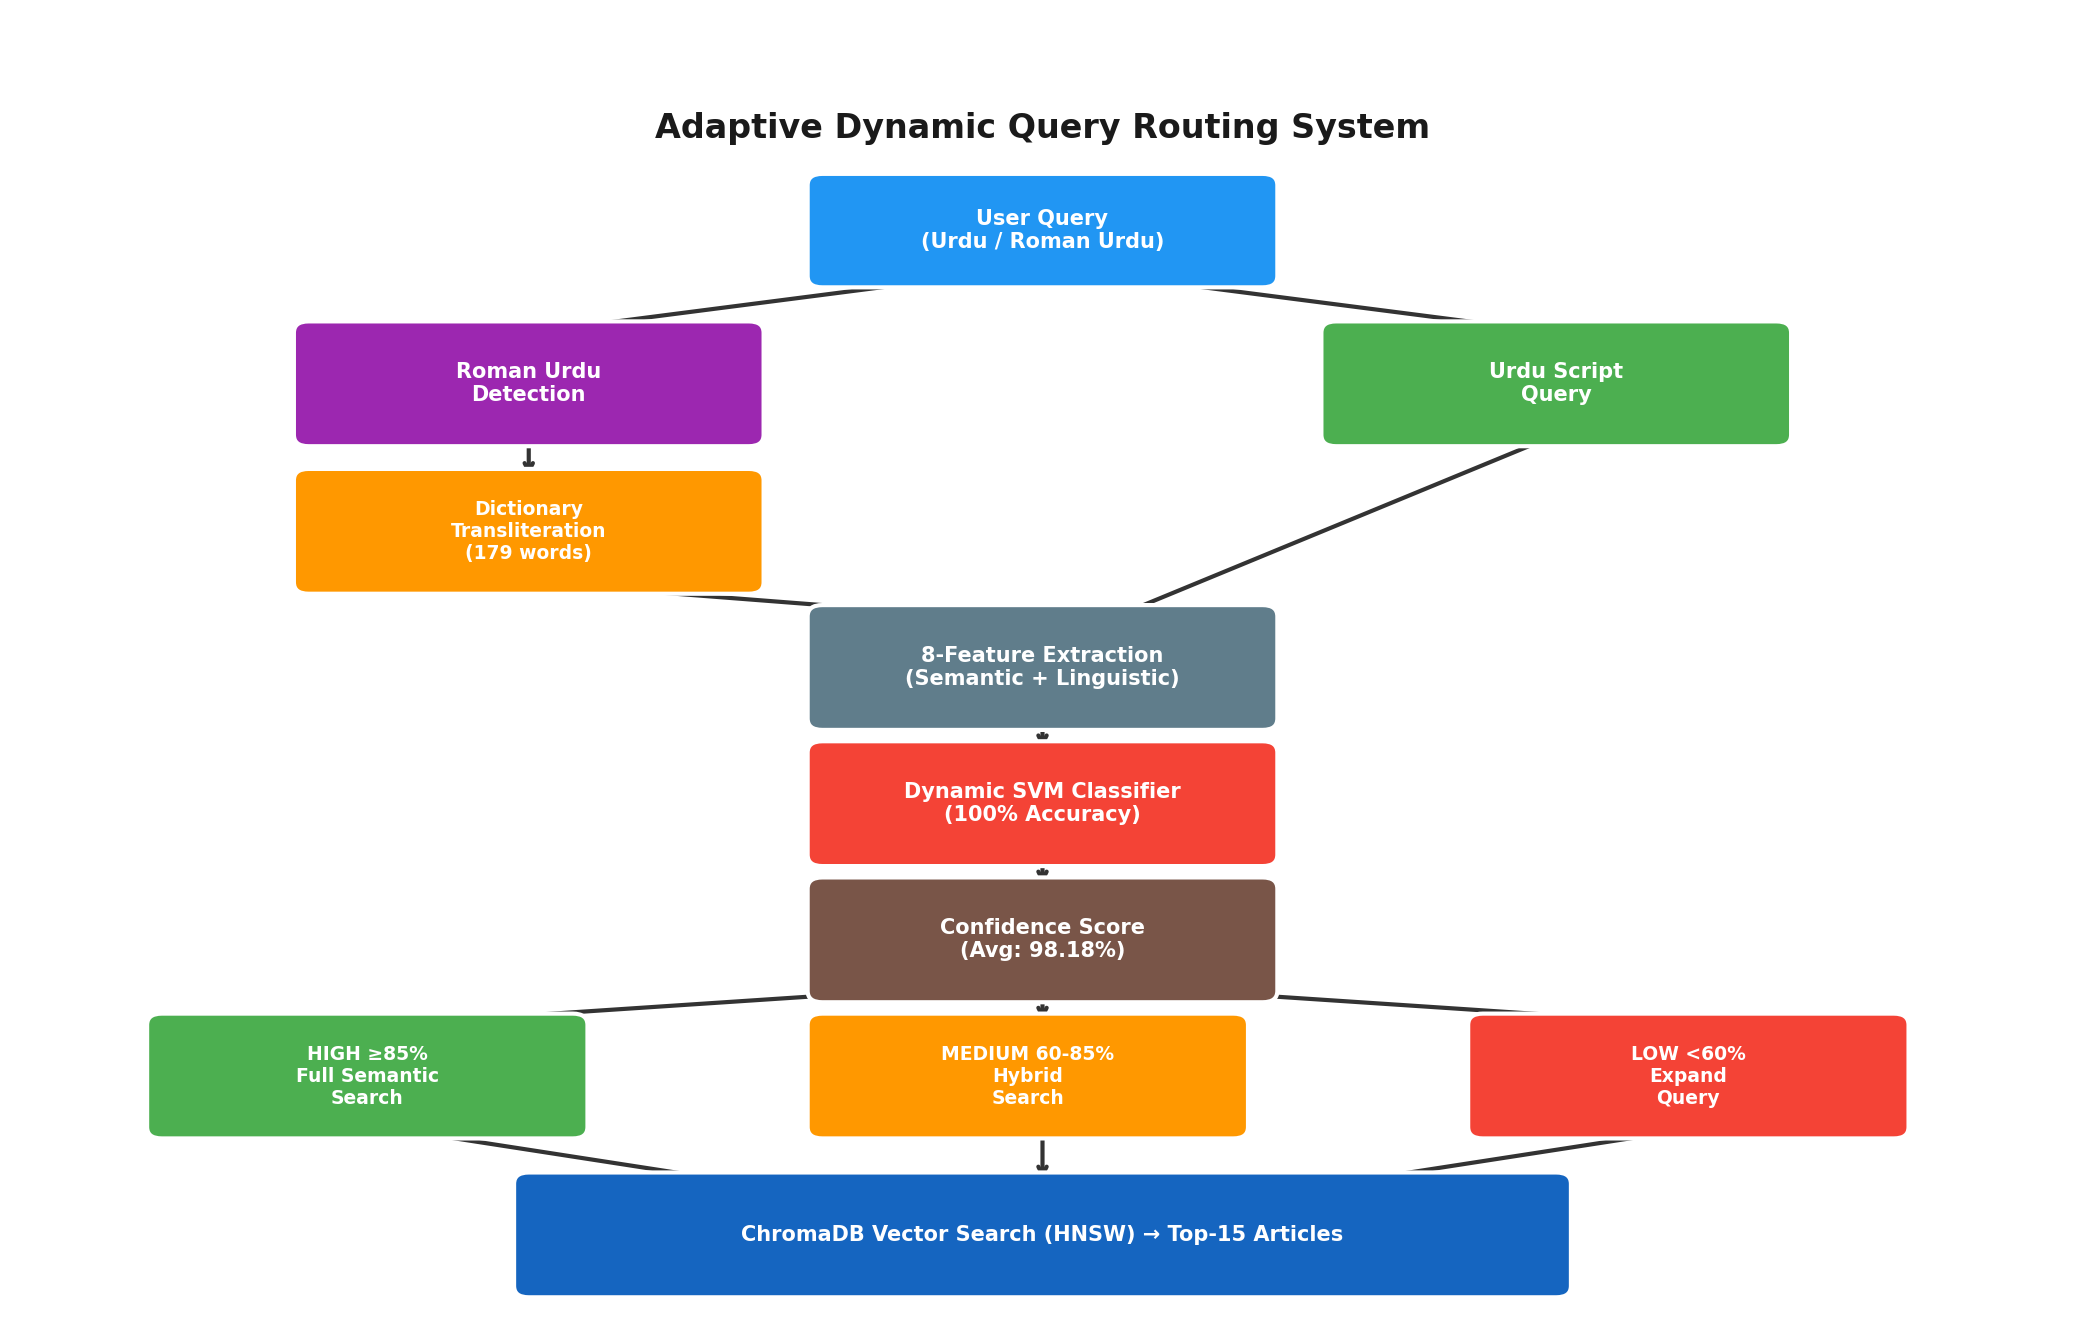
\includegraphics[width=\linewidth]{figures/system_architecture.png}
\caption{\textbf{Development pipeline diagram} (legacy notebook figure). Retrieval in the frozen tests uses two indexes, not a single Chroma search for every query. See Fig~\ref{fig:two_rooms}.}
\label{fig:architecture}
\end{figure}

\begin{figure}[H]
\centering
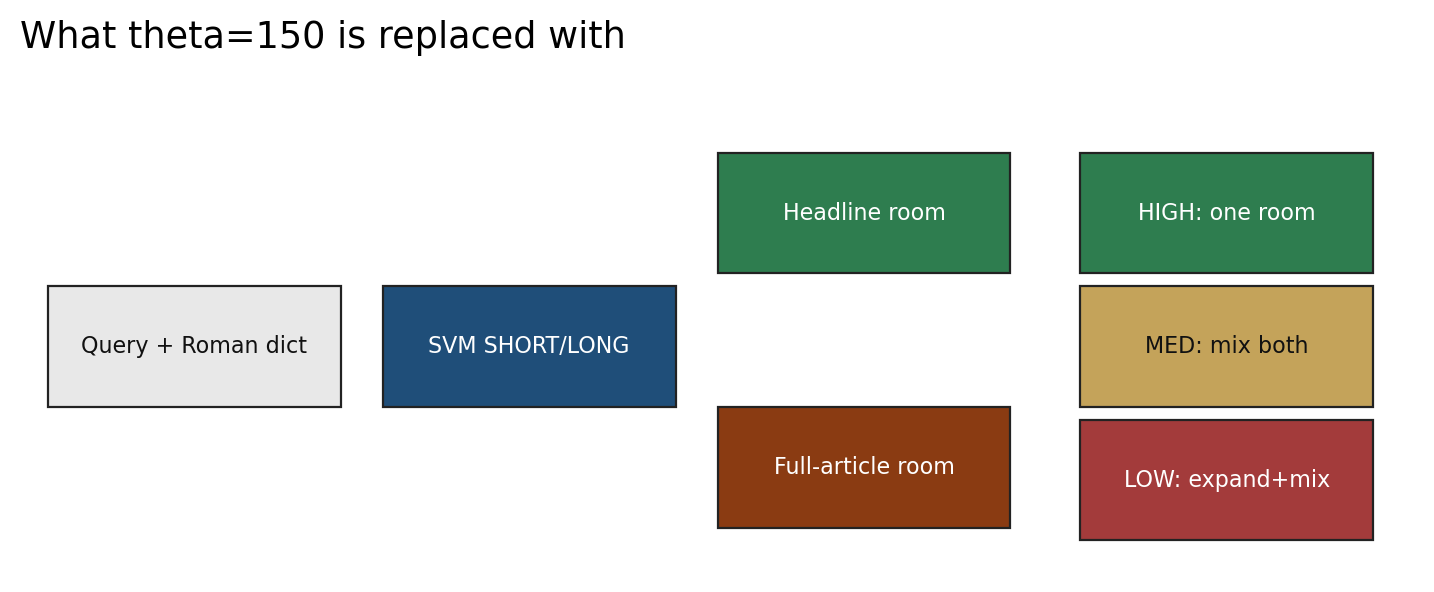
\includegraphics[width=\linewidth]{figures/two_rooms_lights.png}
\caption{\textbf{What the router actually does.} SHORT opens the headline room. LONG opens the full-article room. HIGH confidence stays in one room. MEDIUM mixes both. LOW expands the query and then mixes.}
\label{fig:two_rooms}
\end{figure}

Roman Urdu is mapped with a word list. The file on disk has 198 pairs (older drafts said 179). Native-script Urdu skips that step.

\subsection*{Corpus and indexes}
\label{sec:dataset}

The collection is 111,860 Urdu news articles (Kaggle Urdu News), embedded with \texttt{paraphrase-multilingual-MiniLM-L12-v2} \cite{reimers2019sbert} (384 dimensions) and stored in ChromaDB (\texttt{urdu\_news}) with HNSW and cosine similarity. That store is the full-article room. The headline room is a separate dense index over titles. Both rooms use the same encoder. We did not retrain it after seeing scores.

\begin{table}[H]
\centering
\caption{\textbf{Corpus category breakdown (111,860 articles).}}
\label{tab:corpus_categories}
\small
\begin{tabular}{lcc}
\toprule
\textbf{Category} & \textbf{Articles} & \textbf{\%} \\
\midrule
Sports & 44,829 & 40.07\% \\
Entertainment & 34,901 & 31.21\% \\
Business \& Economics & 24,131 & 21.57\% \\
Science \& Technology & 7,999 & 7.15\% \\
\bottomrule
\end{tabular}
\end{table}

Table~\ref{tab:dataset_summary} lists the query sets we actually freeze. They are not one pool.

\begin{table}[H]
\centering
\caption{\textbf{Query sets used in this paper. Do not average them.}}
\label{tab:dataset_summary}
\small
\begin{tabular}{p{4.2cm} p{6.2cm}}
\toprule
\textbf{Set} & \textbf{Role} \\
\midrule
Development / CV (369--409 labeled queries) & Shows the task is learnable. Some splits hit 100\% vs 50\% for $\theta=150$. Not the paper headline. \\
Frozen Phase 3B, V2, 8 features & 50 primary queries. SVM 86\% vs word count $\geq 6$ at 84\%. \\
Frozen traps H001--H040 & Need labels. Never used to train V2. Classification and dual-index P@5. \\
Phase 2.5 & 33 queries, P@5 depth 5. Supporting only. \\
Roman Urdu dictionary & 198 pairs on disk. \\
\bottomrule
\end{tabular}
\end{table}

Fig~\ref{fig:query_dist} is the development length plot. It still makes the basic point: almost nothing reaches 150 characters, so $\theta=150$ is a dead switch on this query mix.

\begin{figure}[H]
\centering
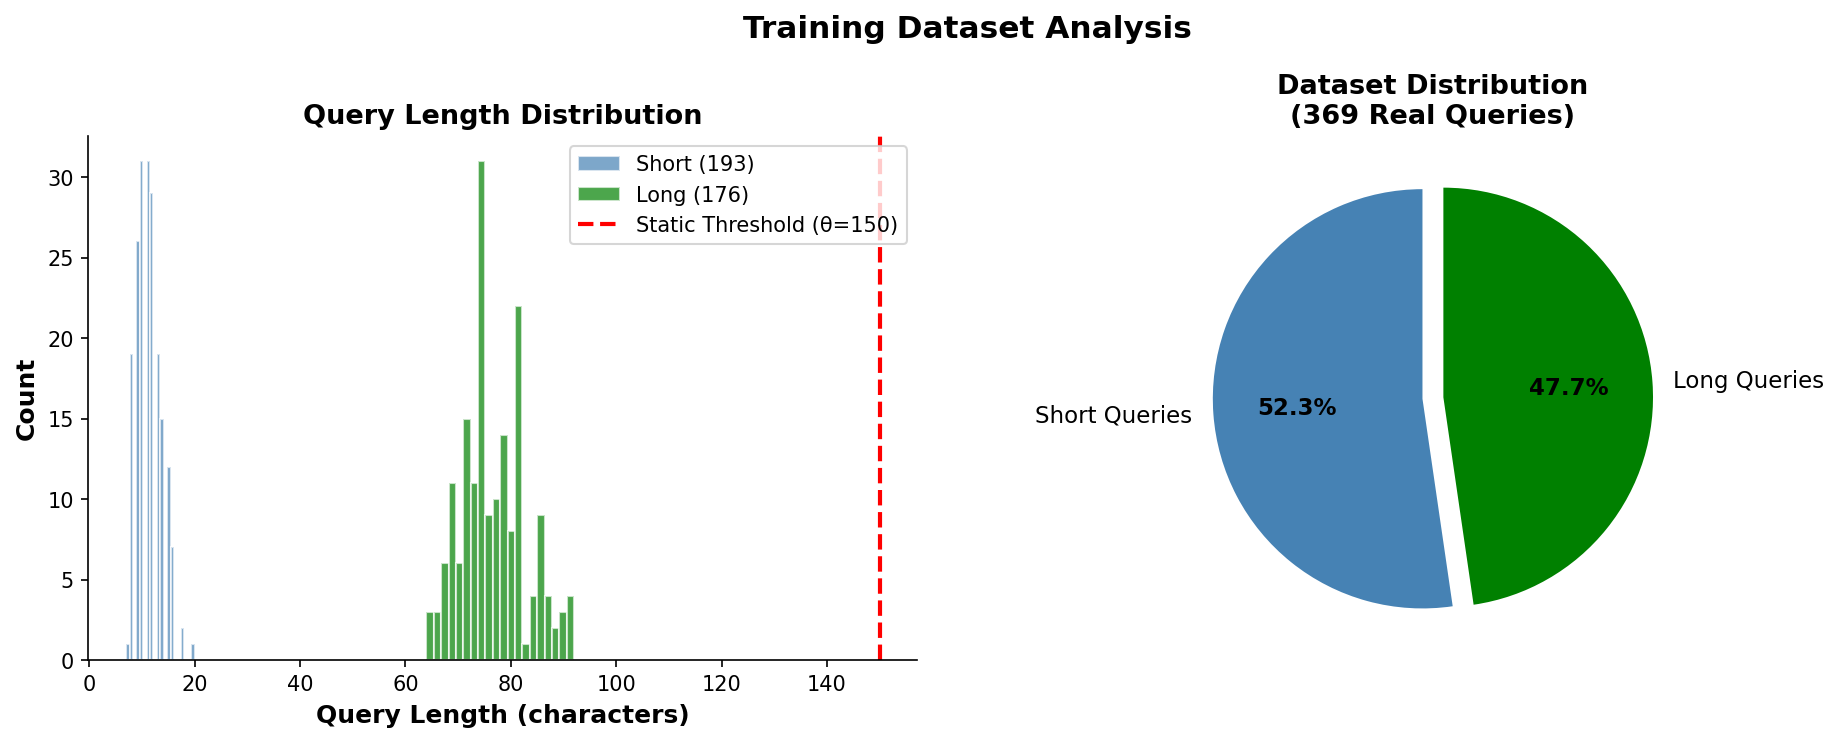
\includegraphics[width=\linewidth]{figures/query_distribution.png}
\caption{\textbf{Development query lengths vs.\ $\theta=150$.} Most queries sit well below the cutoff. That is why the static rule collapses to SHORT.}
\label{fig:query_dist}
\end{figure}

\subsection*{What SHORT and LONG mean}
\label{sec:labels}

SHORT means a headline could answer the user (score, price, date, who won). LONG means they asked for why, how, impact, or a story. We did not label by token count. If we had, we could never beat a six-word rule.

\subsection*{Eight-feature SVM (frozen V2)}
\label{sec:features}

The frozen generalization model uses eight features:

\begin{equation}
\mathbf{x}(q) = \big[x_1(q),\ldots,x_8(q)\big] \in \mathbb{R}^{8}
\label{eq:featurevec}
\end{equation}

\begin{table}[H]
\centering
\caption{\textbf{Frozen V2 feature vector (Phase 3B).}}
\label{tab:features}
\small
\begin{tabular}{clp{4.2cm}}
\toprule
\textbf{\#} & \textbf{Feature} & \textbf{Definition} \\
\midrule
$x_1$ & \texttt{urdu\_ratio} & Share of Urdu-script characters \\
$x_2$ & \texttt{roman\_ratio} & Share of Latin-script characters \\
$x_3$ & \texttt{has\_urdu} & Binary: any Urdu character \\
$x_4$ & \texttt{has\_roman} & Binary: any Latin letter \\
$x_5$ & \texttt{query\_len} & Whitespace token count \\
$x_6$ & \texttt{char\_len} & Character count \\
$x_7$ & \texttt{mixed} & Both scripts present \\
$x_8$ & \texttt{urdu\_chars} & Count of Urdu characters \\
\bottomrule
\end{tabular}
\end{table}

Features are z-scored on the training split only \cite{cortes1995svm}. The SVM uses an RBF kernel. Class probability is Platt scaling \cite{guo2017calibration}:

\begin{equation}
C(q) = \sigma\big(A f(\mathbf{z}(q)) + B\big) \times 100\%
\label{eq:confidence}
\end{equation}

A later twelve-feature pickle exists in the demo. It is not the Phase 3B scorer. Mixing the two is how a 96\% figure appears. We do not report 96\%.

\subsection*{Lights, then rooms}
\label{sec:tiered_routing}

\begin{equation}
R(q) =
\begin{cases}
\text{chosen room only}, & C(q) \geq 85\% \quad \text{(HIGH)} \\[4pt]
\text{mix both rooms}, & 60\% \leq C(q) < 85\% \quad \text{(MEDIUM)} \\[4pt]
\text{expand, then mix}, & C(q) < 60\% \quad \text{(LOW)}
\end{cases}
\label{eq:routing}
\end{equation}

\begin{table}[H]
\centering
\caption{\textbf{Confidence lights.}}
\label{tab:routing_tiers}
\small
\begin{tabular}{llp{5.2cm}}
\toprule
\textbf{Light} & \textbf{$C(q)$} & \textbf{Search} \\
\midrule
HIGH & $\geq 85\%$ & Headline room if SHORT, full-article room if LONG \\
MEDIUM & $60$--$85\%$ & Mix both rooms \\
LOW & $< 60\%$ & Expand query, then mix \\
\bottomrule
\end{tabular}
\end{table}

LOW is implemented. On the small live probe we used for defense it did not fire. We do not pretend that it did.

Similarity in each room is cosine on MiniLM vectors, same as ULTRA's backend:

\begin{equation}
\mathrm{sim}(\mathbf{e}_q, \mathbf{e}_d)
= \frac{\mathbf{e}_q \cdot \mathbf{e}_d}{\lVert\mathbf{e}_q\rVert\,\lVert\mathbf{e}_d\rVert}.
\label{eq:cosine}
\end{equation}

\subsection*{Baselines}
\label{sec:baselines}

Frozen comparisons: $\theta=150$; word count $\geq 6$ tokens $\rightarrow$ LONG; always-headline; always-full-article; the V2 SVM. Development notebooks also compared LLM-style routers on 14 queries. Those numbers stay in the development layer. They are not frozen P@5.

\subsection*{Evaluation}
\label{sec:eval_metrics}

Classification: accuracy and exact McNemar tests. Retrieval: P@5 and nDCG@5 on 400 graded judgments (40 queries $\times$ 5). Phase 2.5 used 33 queries at depth 5. We do not convert a McNemar $p=1$ into a win speech.

\begin{figure}[H]
\centering
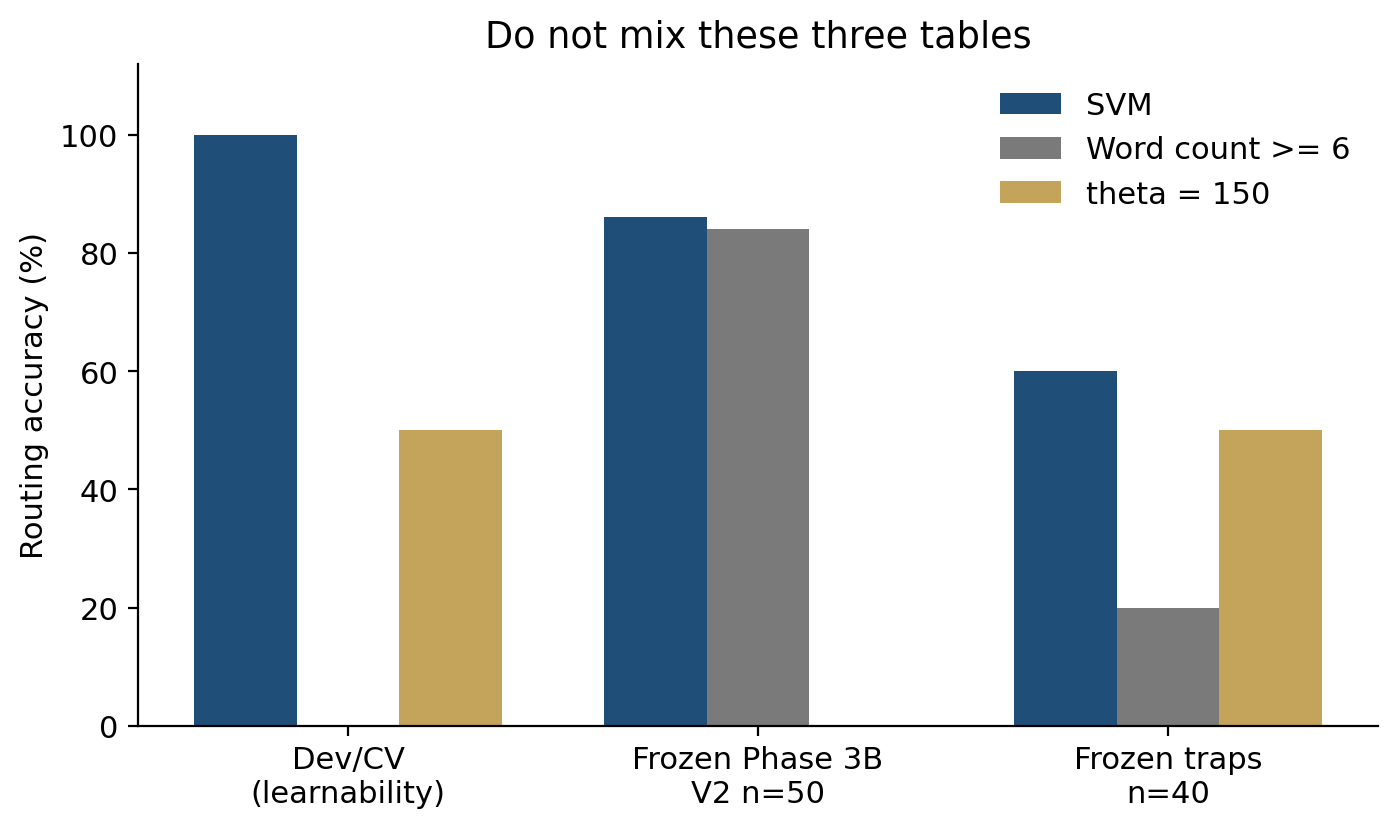
\includegraphics[width=\linewidth]{figures/three_evaluation_layers.png}
\caption{\textbf{Three layers that must not be mixed:} development/CV, frozen Phase 3B (86/84), frozen traps (60/20/50 and P@5).}
\label{fig:layers}
\end{figure}

% ============================================================
\section*{Results}
\label{sec:results}
% ============================================================

\subsection*{Development routing looks solved. That is not the claim.}
\label{sec:res_accuracy}

On development splits the SVM can hit 100\% while $\theta=150$ sits at 50\% (Table~\ref{tab:routing_accuracy}, Fig~\ref{fig:confusion_matrix}). Fig~\ref{fig:perf_comparison} is from that same notebook era. We keep the figures because they show learnability. We do not keep them as the generalization headline.

\begin{table}[H]
\centering
\caption{\textbf{Development routing accuracy (not frozen Phase 3B).}}
\label{tab:routing_accuracy}
\small
\begin{tabular}{lc}
\toprule
\textbf{Method} & \textbf{Accuracy} \\
\midrule
Static threshold ($\theta=150$) & 50.00\% \\
Logistic regression (dev split) & 100.00\% \\
SVM, RBF (dev split) & 100.00\% \\
\bottomrule
\end{tabular}
\end{table}

\begin{figure}[H]
\centering
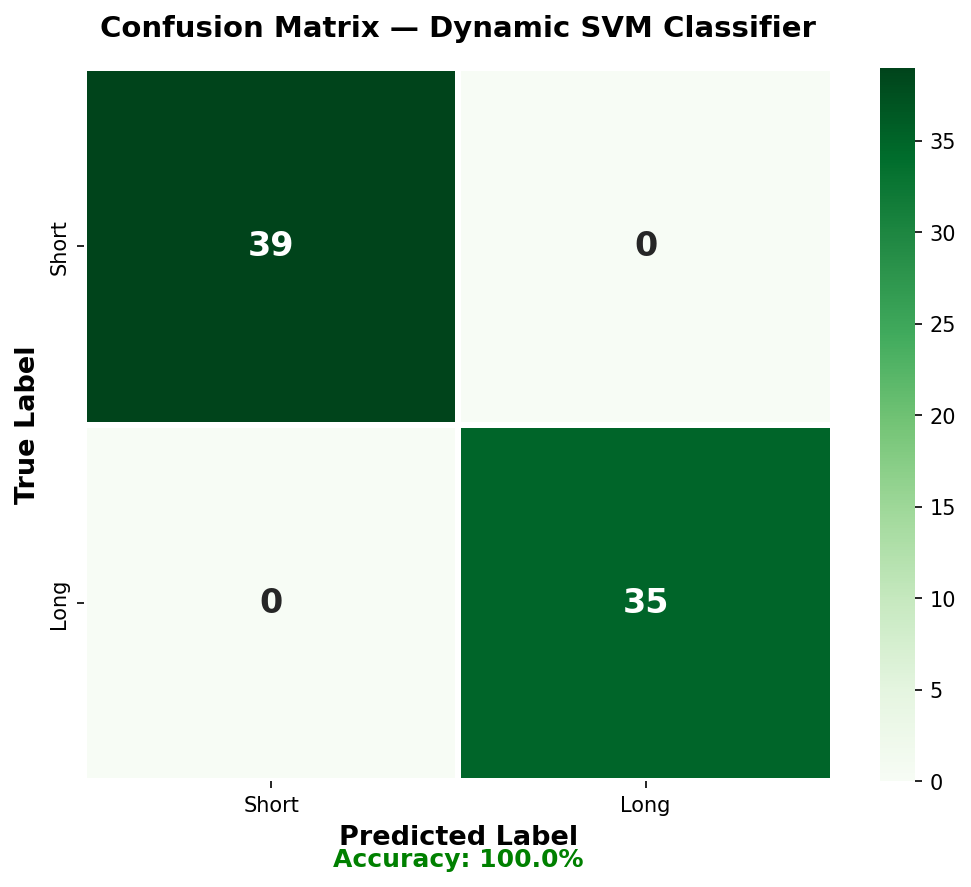
\includegraphics[width=\linewidth]{figures/confusion_matrix.png}
\caption{\textbf{Development confusion matrix} (74-query split). Treat as learnability, not as the frozen test.}
\label{fig:confusion_matrix}
\end{figure}

\begin{figure}[H]
\centering
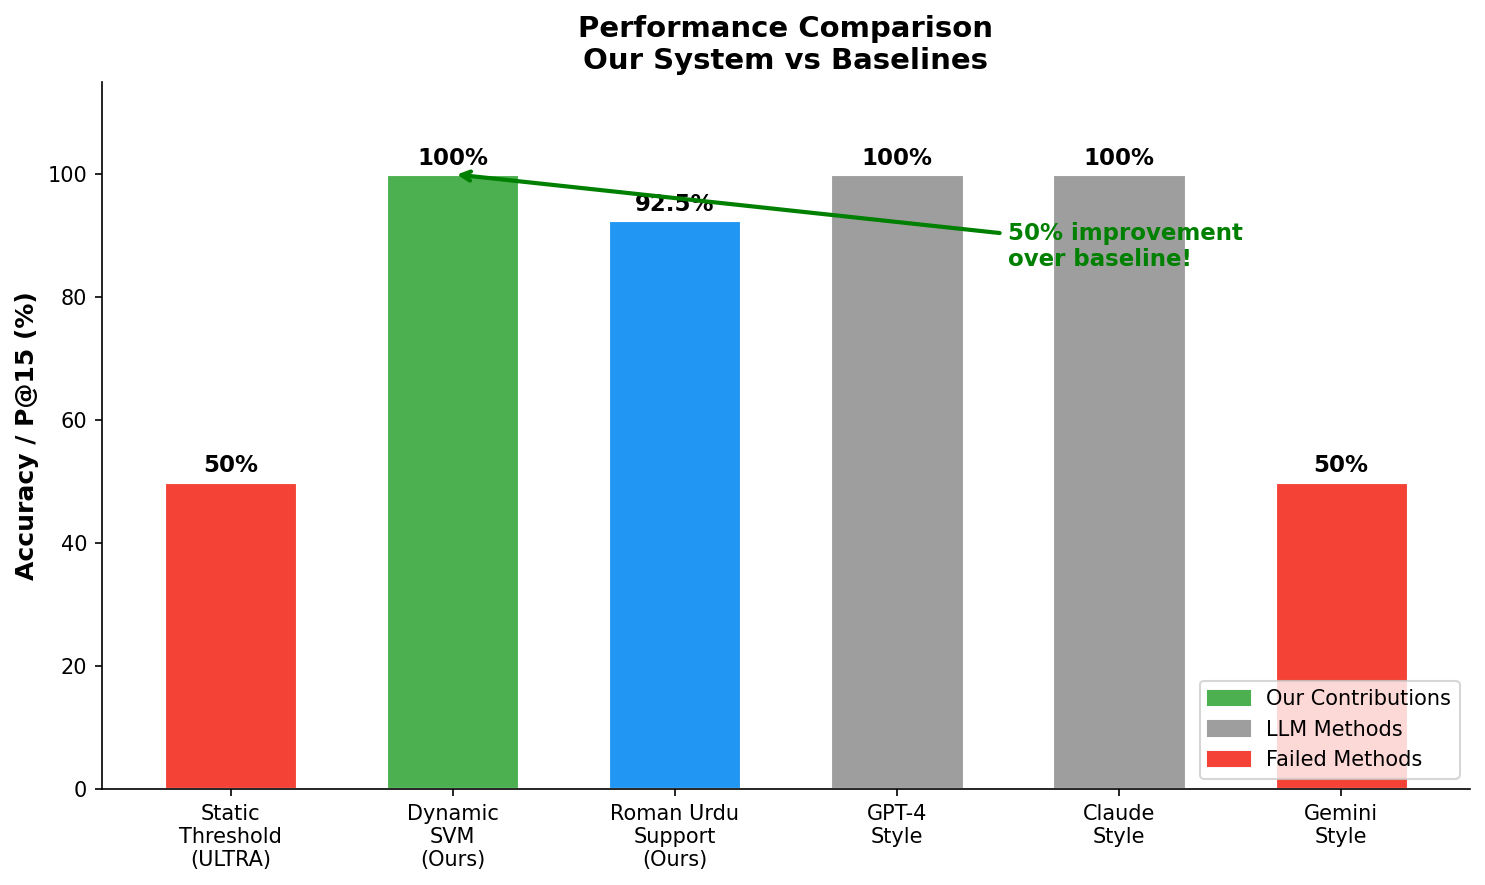
\includegraphics[width=\linewidth]{figures/performance_comparison.png}
\caption{\textbf{Development performance panel.} Do not quote this as the held-out result.}
\label{fig:perf_comparison}
\end{figure}

\subsection*{Frozen Phase 3B: 86\% vs 84\%}
\label{sec:res_p15}

On 50 primary queries the V2 SVM was right 43 times (86\%). Word count was right 42 times (84\%). McNemar is 2 vs 1, exact $p=1.0$. If this were the only experiment, the paper would be thin. It is a check that the frozen extractor matches the trained V2 model.

\subsection*{Frozen traps: a classification gap, with a catch}
\label{sec:res_traps}

On H001--H040 the SVM reached 60\%, word count 20\%, $\theta=150$ 50\%. McNemar vs word count is 16--0 ($p<0.001$).

The cue split is the part that should stay on the slide (Fig~\ref{fig:cue}). Eighteen queries fire why/how/fact wording: SVM 18/18, word count 2/18. The other 22 do not fire those cues: both systems 27.27\%. So the trap win is not ``the SVM understands need.'' It is ``the SVM notices certain words, and the traps were rich in those words.''

\begin{table}[H]
\centering
\caption{\textbf{Frozen classification. Do not mix with development 100\%.}}
\label{tab:frozen_cls}
\small
\begin{tabular}{lccc}
\toprule
\textbf{Layer} & \textbf{SVM} & \textbf{Word count} & \textbf{$\theta=150$} \\
\midrule
Phase 3B ($n=50$) & 86\% & 84\% & -- \\
Traps ($n=40$) & 60\% & 20\% & 50\% \\
Traps with cue ($n=18$) & 100\% & 11.11\% & -- \\
Traps, no cue ($n=22$) & 27.27\% & 27.27\% & -- \\
\bottomrule
\end{tabular}
\end{table}

\begin{figure}[H]
\centering
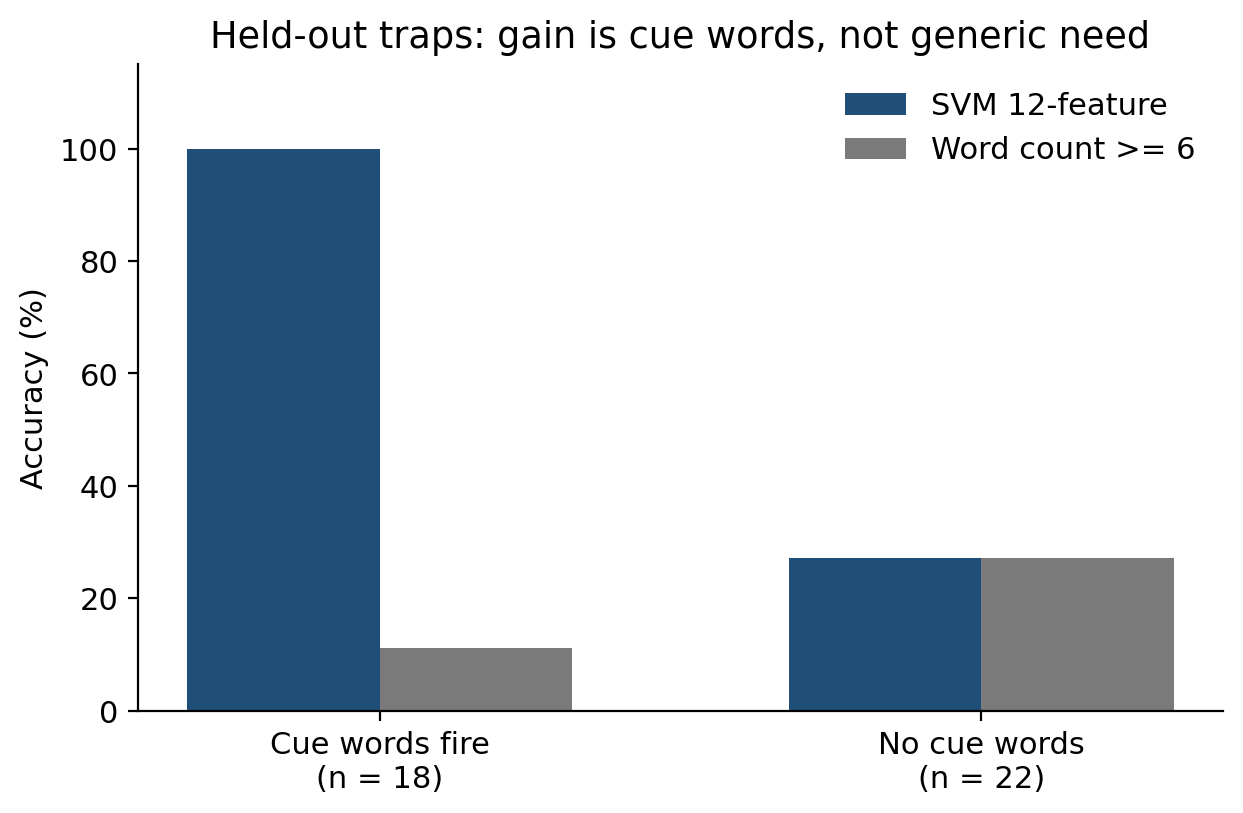
\includegraphics[width=\linewidth]{figures/cue_split.png}
\caption{\textbf{Trap cue split ($n=40$).} SVM 18/18 when why/how/fact wording fires; 27.27\% for both systems otherwise.}
\label{fig:cue}
\end{figure}

\subsection*{Dual-index P@5: the classification win does not transfer}
\label{sec:res_p5}

Table~\ref{tab:p5} is the number that almost got cut. On the same 40 queries, word count had the best P@5 (36.50\%). Always-headline and $\theta=150$ tied at 35.00\%. Always-full-article was 34.25\%. The SVM was last at 33.00\%. nDCG@5 ranked always-headline first (0.6868).

\begin{table}[H]
\centering
\caption{\textbf{Frozen dual-index retrieval on H001--H040 (400 judgments, cutoff 5).}}
\label{tab:p5}
\small
\begin{tabular}{lcccc}
\toprule
\textbf{Router} & \textbf{P@5} & \textbf{nDCG@5} & \textbf{$\to$H} & \textbf{$\to$F} \\
\midrule
Word count $\geq 6$ & 36.50\% & 0.6476 & 20 & 20 \\
Always headline / $\theta=150$ & 35.00\% & 0.6868 & 40 & 0 \\
Always full article & 34.25\% & 0.6020 & 0 & 40 \\
SVM (V2) & 33.00\% & 0.6149 & 20 & 20 \\
\bottomrule
\end{tabular}
\end{table}

\begin{figure}[H]
\centering
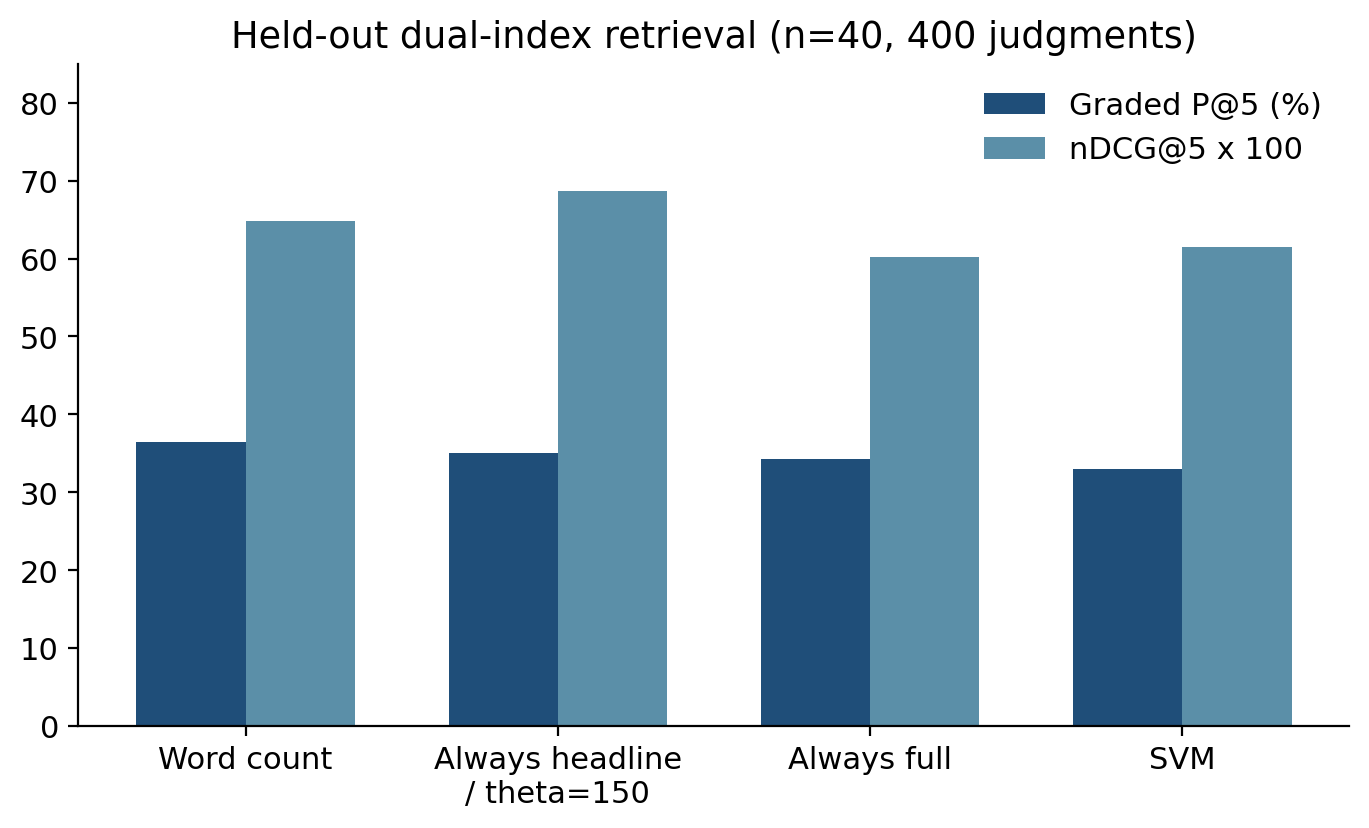
\includegraphics[width=\linewidth]{figures/heldout_p5.png}
\caption{\textbf{Held-out dual-index P@5.} The SVM does not win early precision on this set.}
\label{fig:p5}
\end{figure}

A smaller Phase 2.5 dual-index run ($n=33$) had a tiny SVM edge (35.76\% vs 35.15\% word count vs 32.73\% for $\theta=150$). We do not stack it on the frozen 40 to invent a retrieval win.

Older P@15 Roman Urdu tables (Fig~\ref{fig:roman_urdu_breakdown}, Table~\ref{tab:roman_urdu_individual}) come from the development notebooks. They show the dictionary helping Roman queries that ULTRA used to score at zero by construction. They are not the frozen P@5.

\begin{figure}[H]
\centering
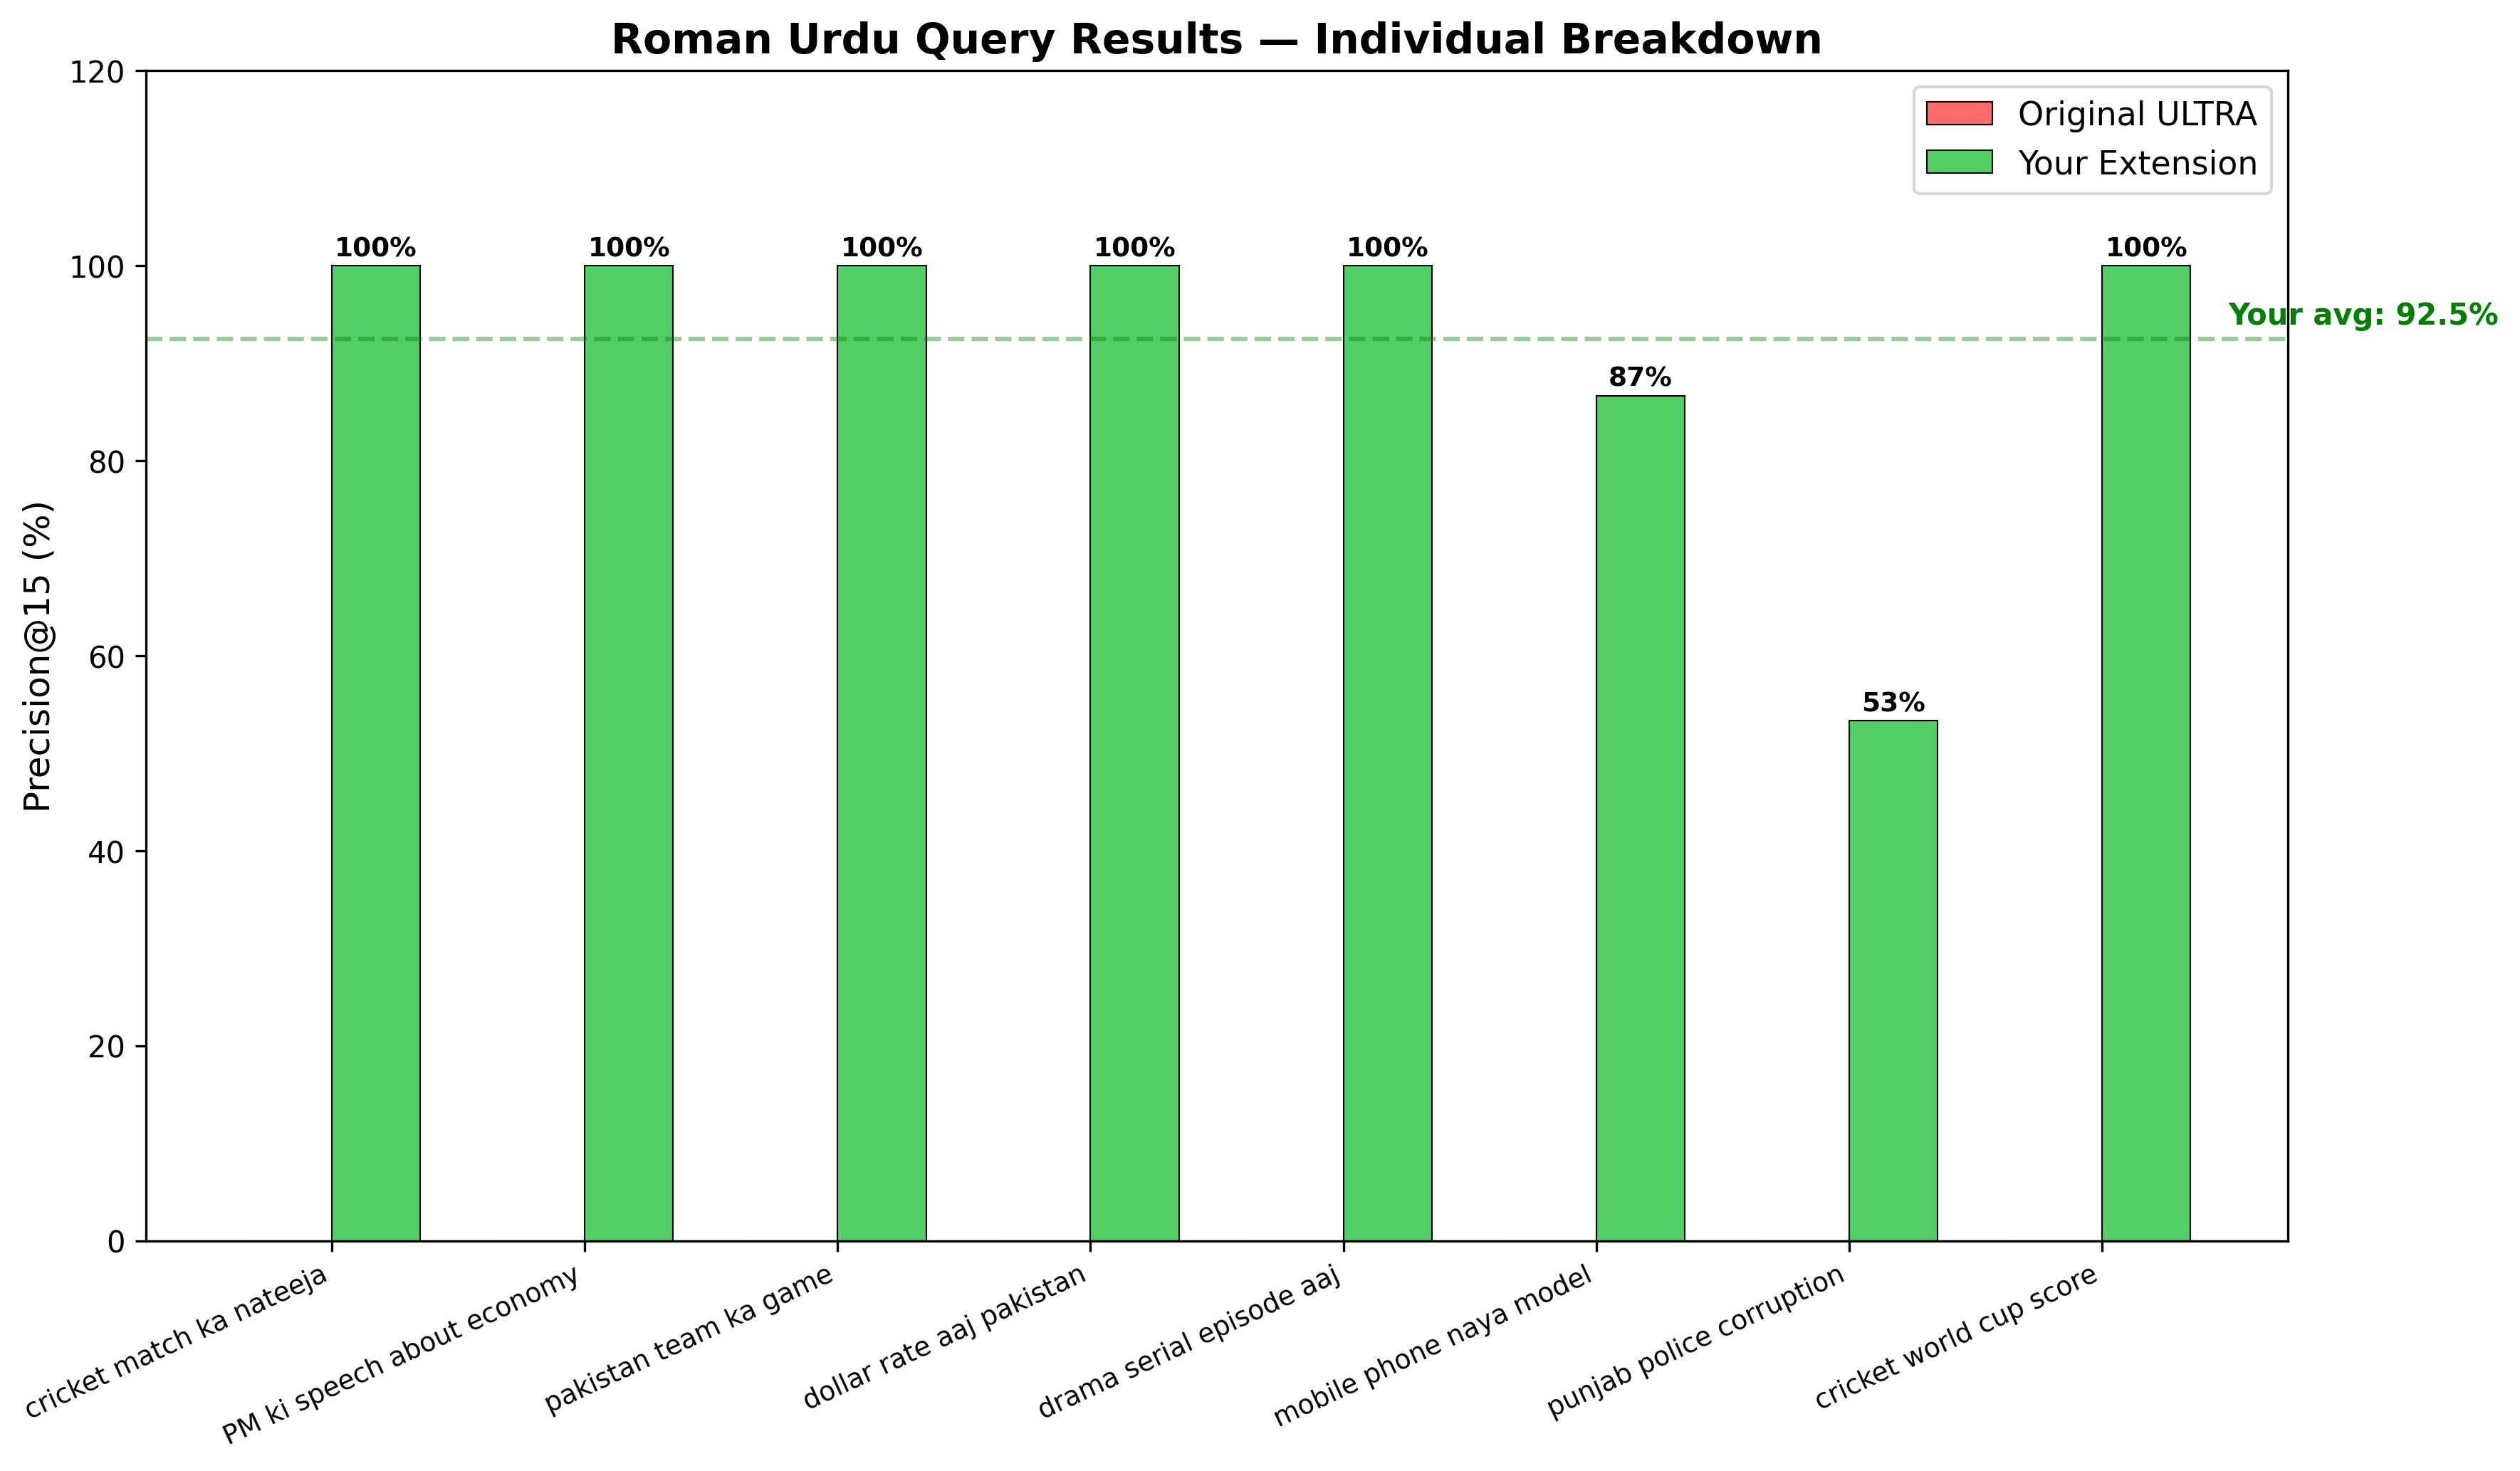
\includegraphics[width=\linewidth]{figures/thesis_chart2_roman_urdu.png}
\caption{\textbf{Development Roman Urdu P@15 breakdown} (8 queries). Supporting dictionary evidence, not the frozen retrieval test.}
\label{fig:roman_urdu_breakdown}
\end{figure}

\begin{table}[H]
\centering
\caption{\textbf{Development Roman Urdu P@15 (8 queries).}}
\label{tab:roman_urdu_individual}
\small
\begin{tabular}{lc}
\toprule
\textbf{Query} & \textbf{P@15} \\
\midrule
cricket match ka nateeja & 100.00\% \\
PM ki speech about economy & 100.00\% \\
pakistan team ka game & 100.00\% \\
dollar rate aaj pakistan & 100.00\% \\
drama serial episode aaj & 100.00\% \\
cricket world cup score & 100.00\% \\
mobile phone naya model & 86.67\% \\
punjab police corruption & 53.33\% \\
\midrule
\textbf{Average} & \textbf{92.50\%} \\
\bottomrule
\end{tabular}
\end{table}

\subsection*{LLM-style routers and other development panels}
\label{sec:res_llm}

Table~\ref{tab:llm_comparison} and Figs~\ref{fig:all_methods}--\ref{fig:efficiency} are development comparisons on 14 queries. Three LLM-style routers match 100\% there; the SVM does it in 0.4555\,ms locally. That is a latency argument, not a frozen accuracy argument.

\begin{table}[H]
\centering
\caption{\textbf{Development LLM-style comparison (14 queries).}}
\label{tab:llm_comparison}
\small
\begin{tabular}{lccc}
\toprule
\textbf{System} & \textbf{Accuracy} & \textbf{Latency} & \textbf{Cost} \\
\midrule
Static threshold & 50.00\% & 0.0004 ms & Free \\
GPT-4 style & 100.00\% & 800 ms & Paid \\
GPT-3.5 style & 100.00\% & 600 ms & Paid \\
Claude style & 100.00\% & 700 ms & Paid \\
Gemini style & 50.00\% & 900 ms & Paid \\
SVM (dev) & 100.00\% & 0.4555 ms & Free \\
\bottomrule
\end{tabular}
\end{table}

\begin{figure}[H]
\centering
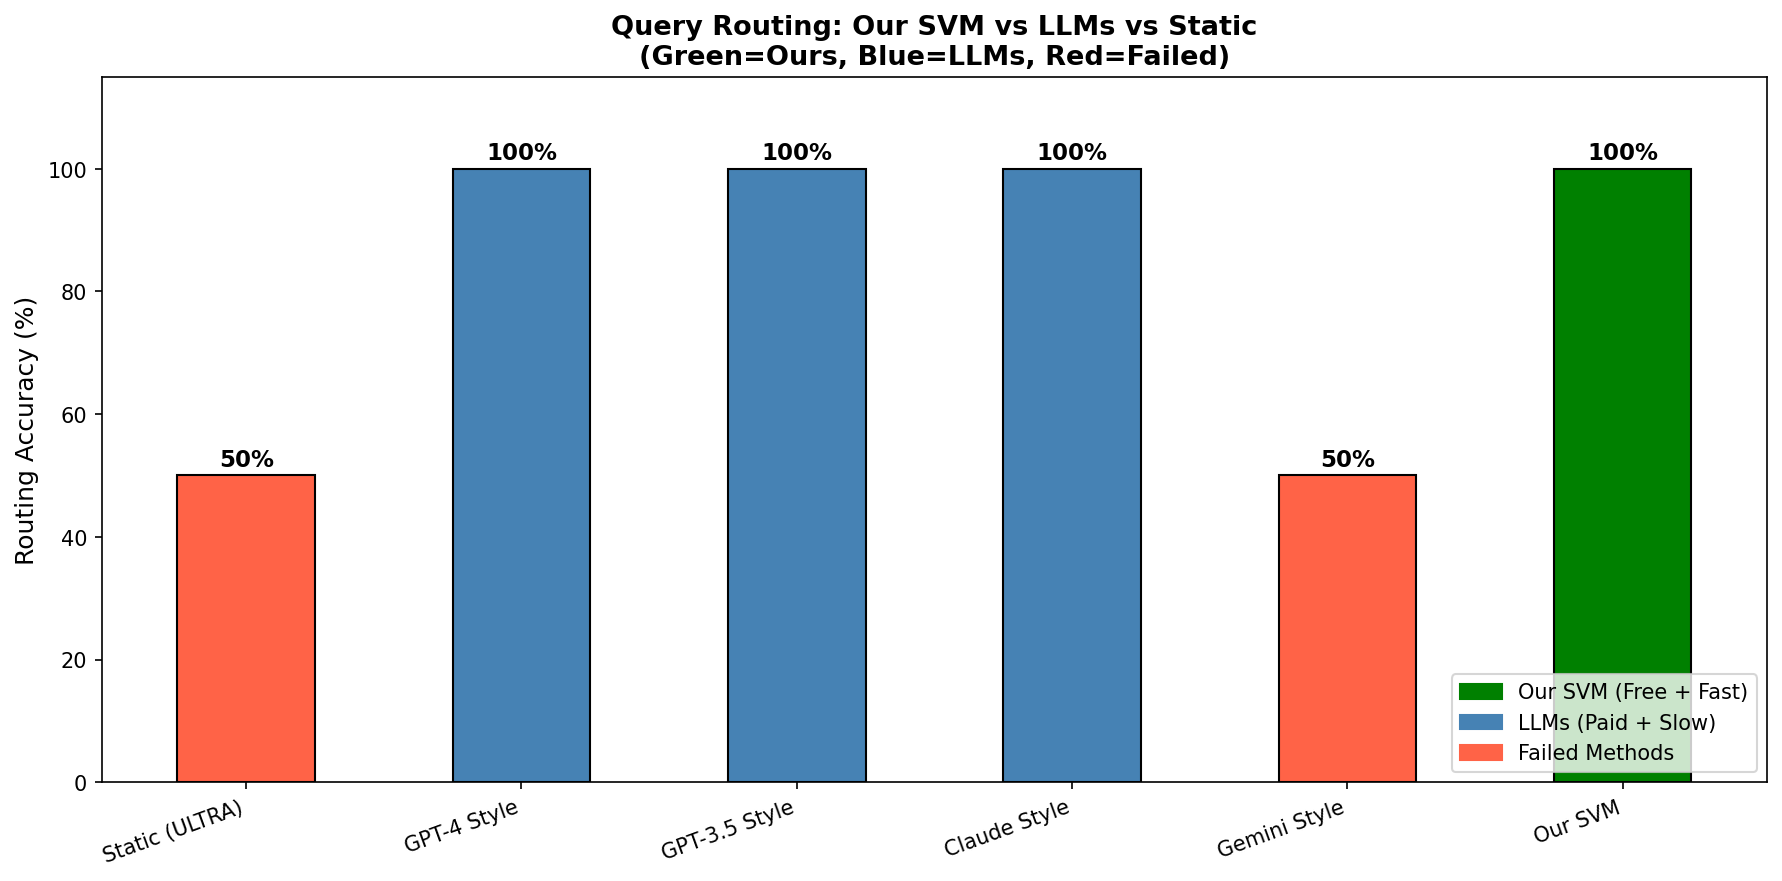
\includegraphics[width=0.95\linewidth]{figures/all_methods_comparison.png}
\caption{\textbf{Development routing accuracy across methods.}}
\label{fig:all_methods}
\end{figure}

\begin{figure}[H]
\centering
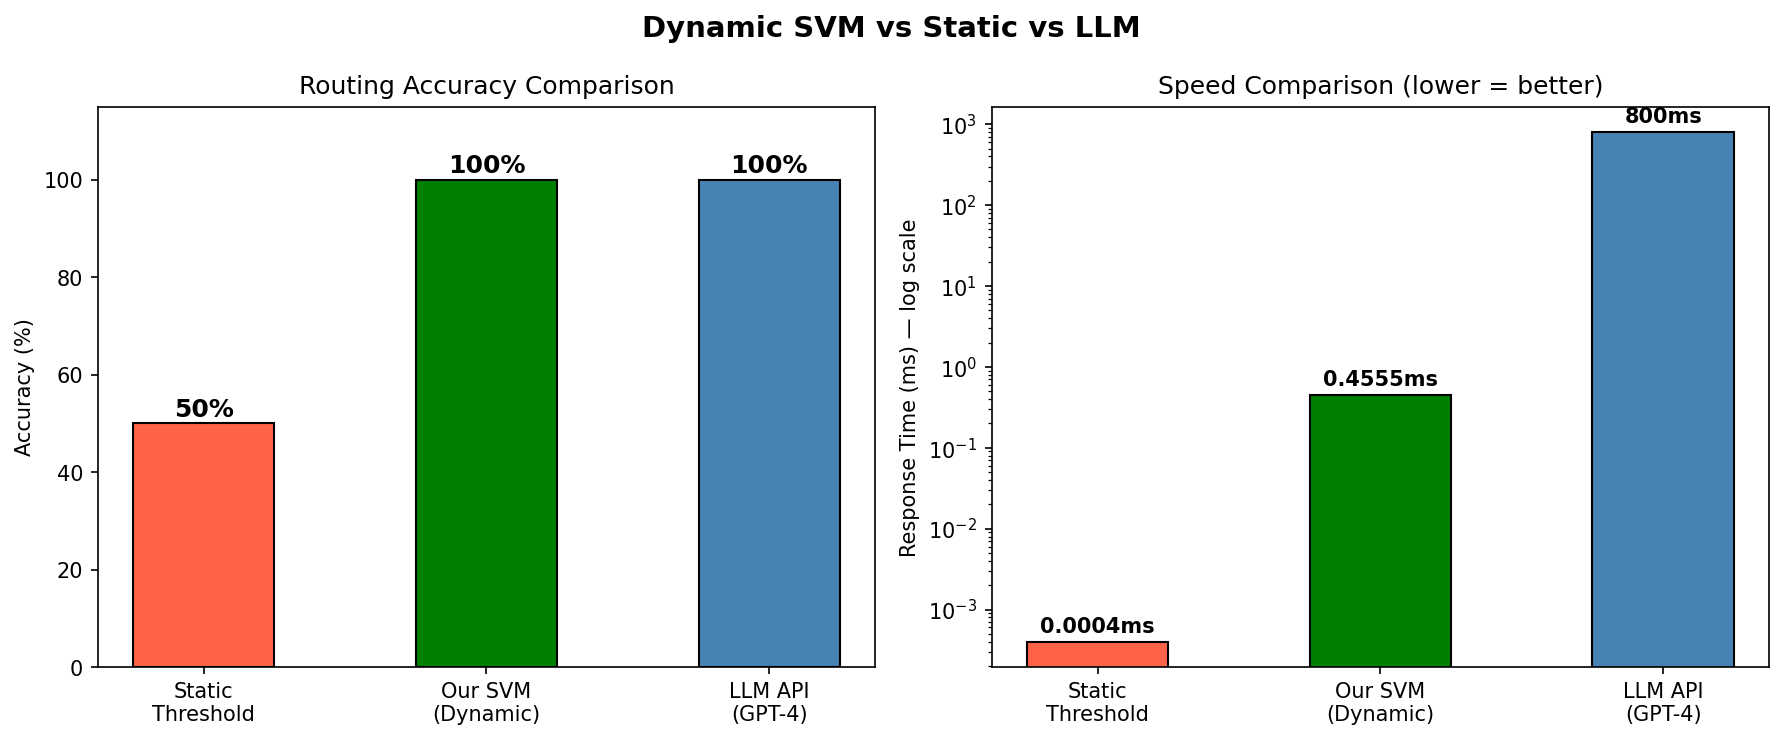
\includegraphics[width=0.95\linewidth]{figures/llm_comparison.png}
\caption{\textbf{Development latency panel (log scale).}}
\label{fig:llm_comparison}
\end{figure}

\begin{figure}[H]
\centering
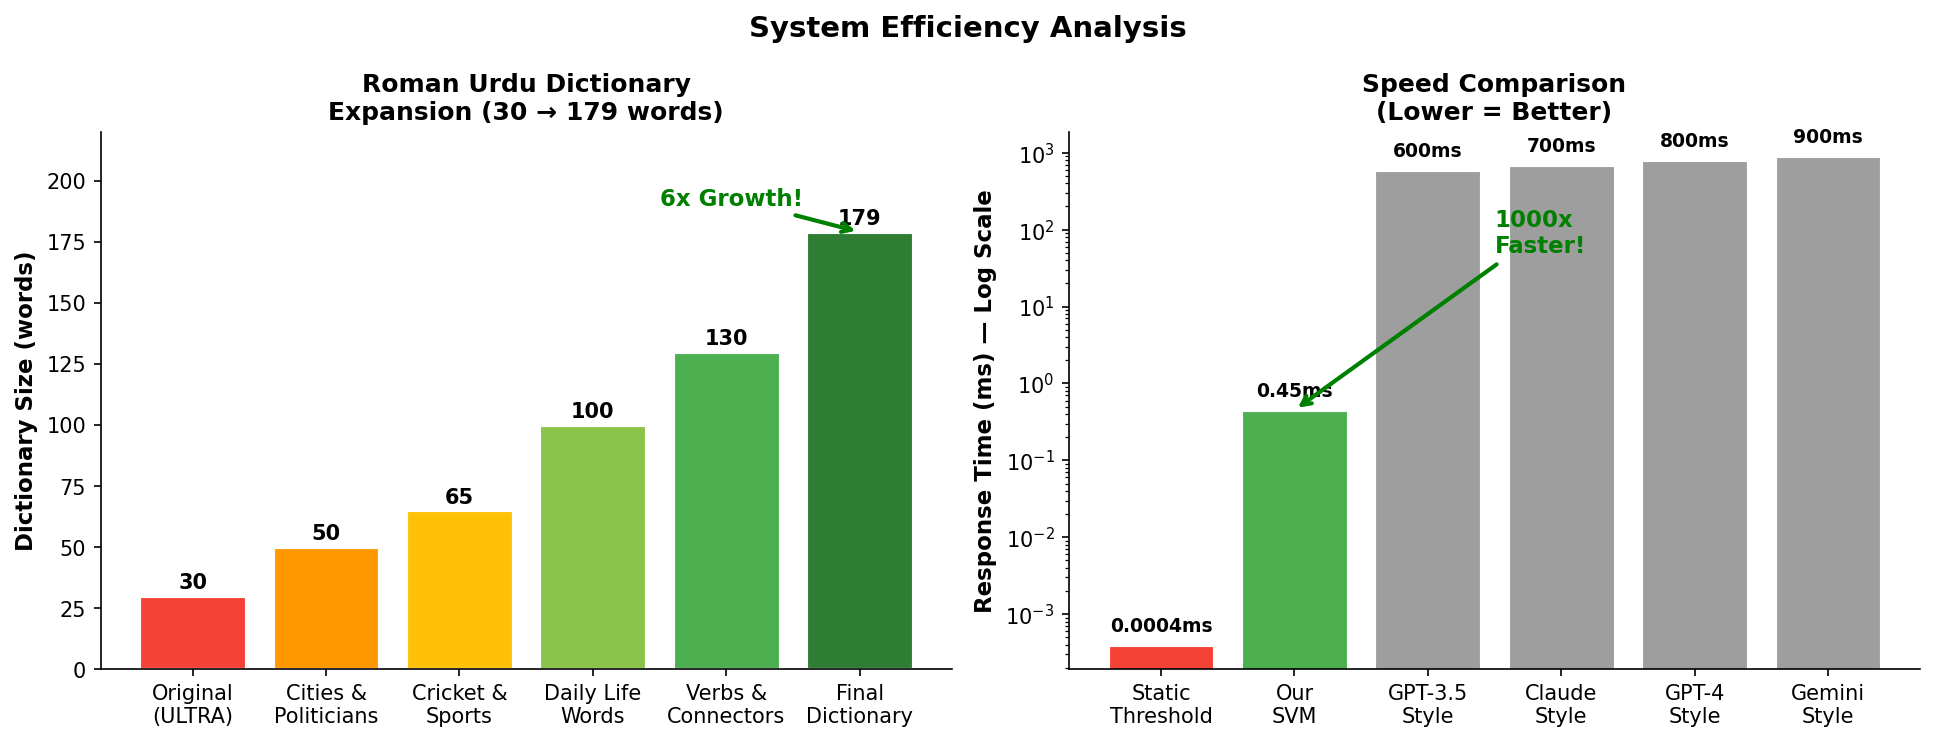
\includegraphics[width=0.95\linewidth]{figures/efficiency_analysis.png}
\caption{\textbf{Development efficiency panel.} Dictionary growth in older drafts was listed as 30 $\to$ 179; the file on disk is 198 pairs.}
\label{fig:efficiency}
\end{figure}

\subsection*{Feature diagnostics (development)}
\label{sec:res_featimp}

Figs~\ref{fig:feature_importance}--\ref{fig:ablation} and Table~\ref{tab:ablation} are development ablations on the old eight-feature notebook set, including \texttt{has\_question\_words}. They explain why length-only routing is brittle. They are not a second frozen test.

\begin{figure}[H]
\centering
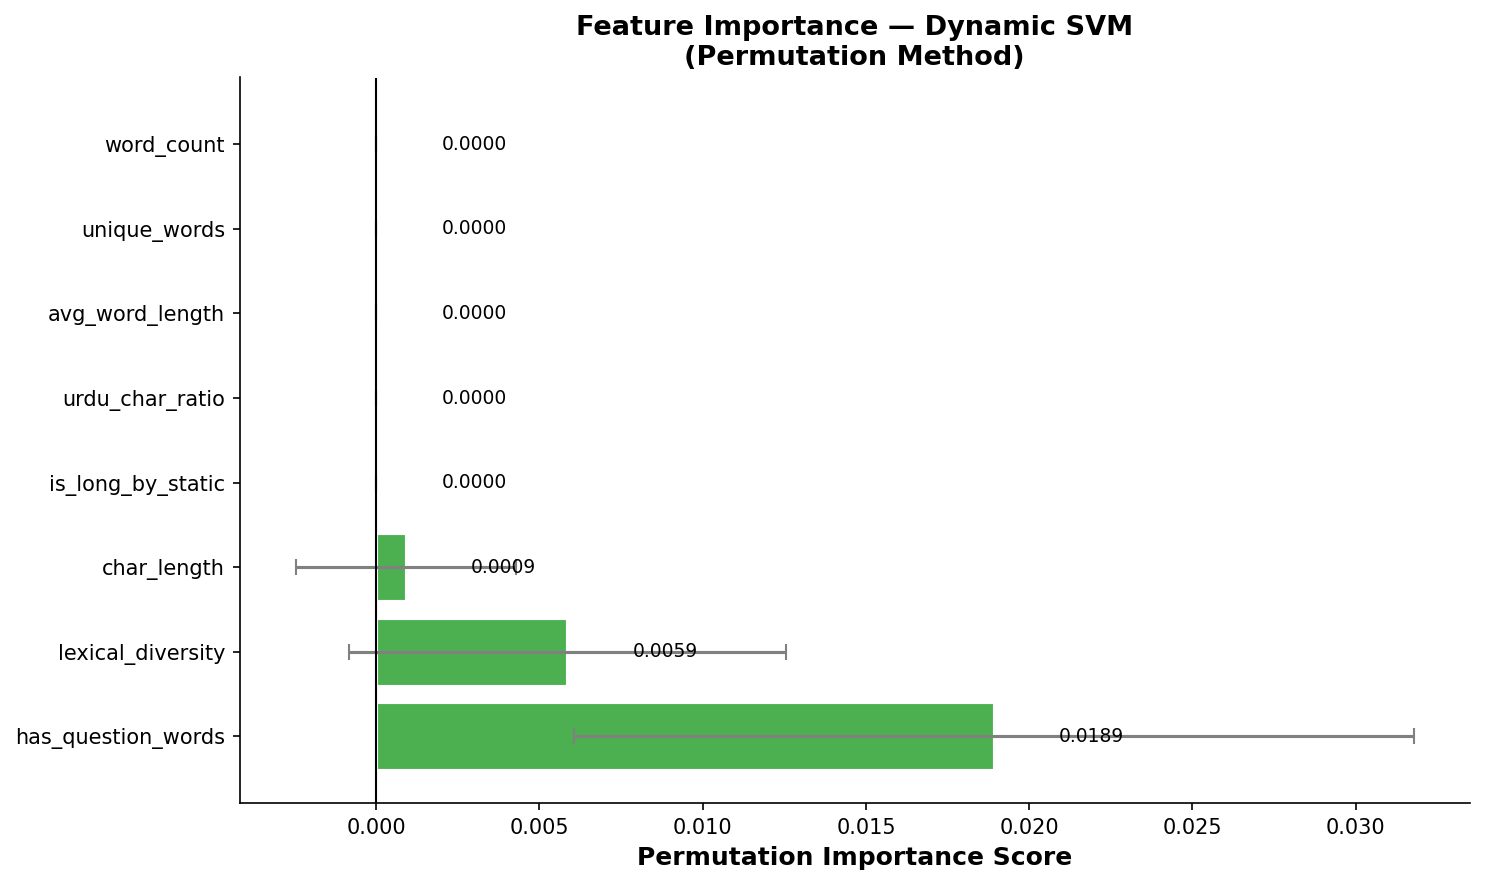
\includegraphics[width=\linewidth]{figures/feature_importance.png}
\caption{\textbf{Development permutation importance.}}
\label{fig:feature_importance}
\end{figure}

\begin{table}[H]
\centering
\caption{\textbf{Development ablation (old 8-feature notebook). All rows at 100\% means the split was easy, not that every feature is useless.}}
\label{tab:ablation}
\small
\begin{tabular}{lcc}
\toprule
\textbf{Configuration} & \textbf{Accuracy} & \textbf{$\Delta$} \\
\midrule
All 8 features & 100.00\% & -- \\
Each leave-one-out & 100.00\% & 0.00\% \\
\bottomrule
\end{tabular}
\end{table}

\begin{figure}[H]
\centering
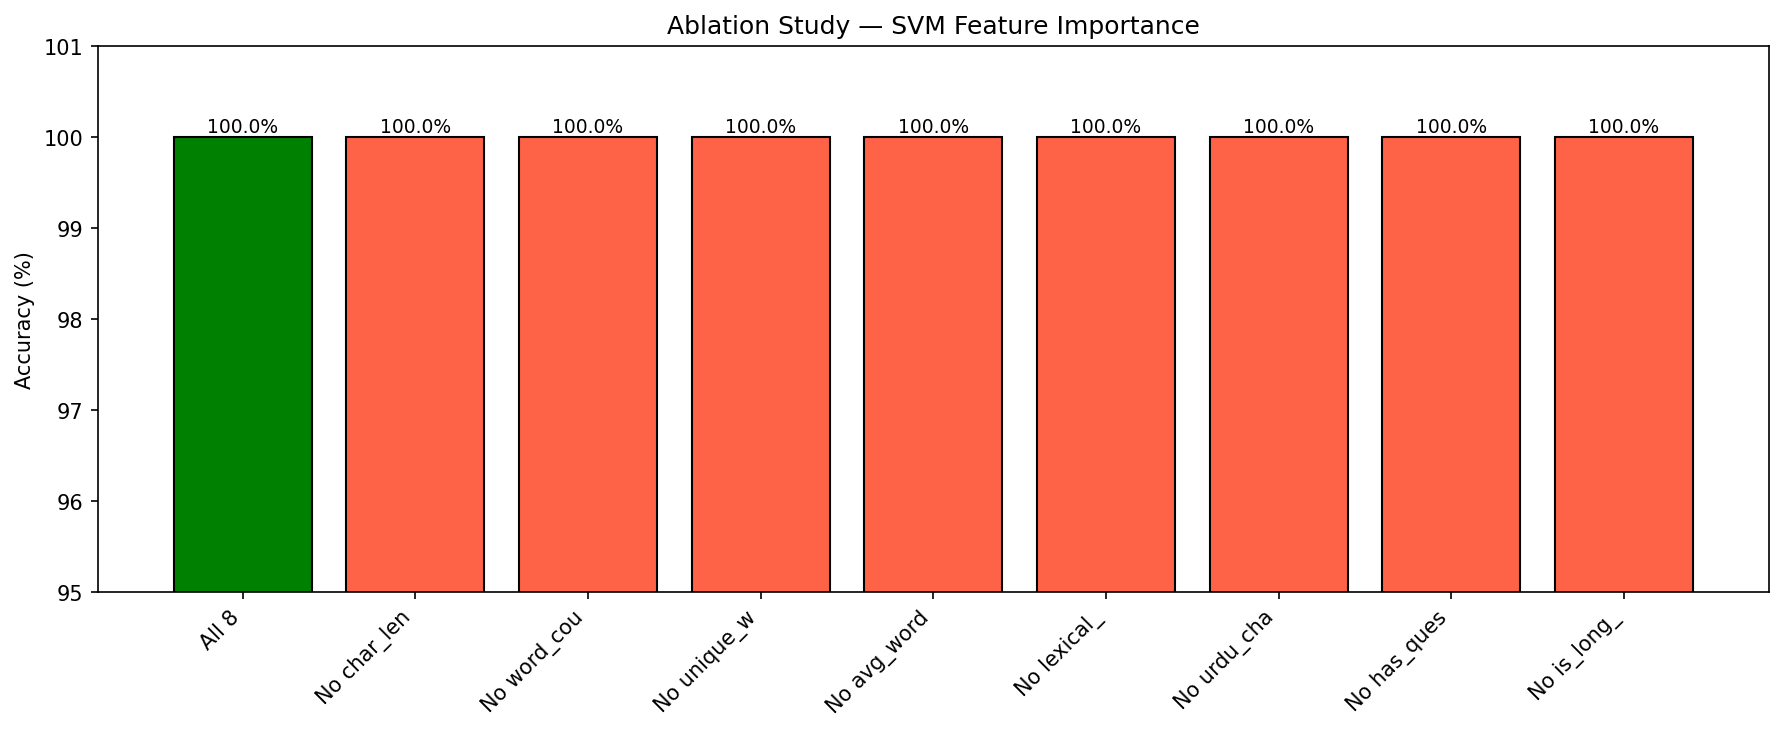
\includegraphics[width=\linewidth]{figures/ablation_study.png}
\caption{\textbf{Development ablation plot.}}
\label{fig:ablation}
\end{figure}

\subsection*{Confidence demo}
\label{sec:res_tierdist}

An 8-query development batch sat entirely in HIGH (Table~\ref{tab:tier_distribution}, Fig~\ref{fig:confidence_routing}), average confidence 98.18\%. The live defense demo is different: cricket match is green; dollar-rise and a stock-exchange query are yellow. We do not recycle an old JSON that painted a score query red.

\begin{table}[H]
\centering
\caption{\textbf{Development 8-query confidence batch (all HIGH).}}
\label{tab:tier_distribution}
\small
\begin{tabular}{lccc}
\toprule
\textbf{Tier} & \textbf{Queries} & \textbf{\%} & \textbf{Action} \\
\midrule
HIGH ($\geq 85\%$) & 8 & 100\% & One room \\
MEDIUM ($60$--$85\%$) & 0 & 0\% & Mix \\
LOW ($< 60\%$) & 0 & 0\% & Expand then mix \\
\bottomrule
\end{tabular}
\end{table}

\begin{figure}[H]
\centering
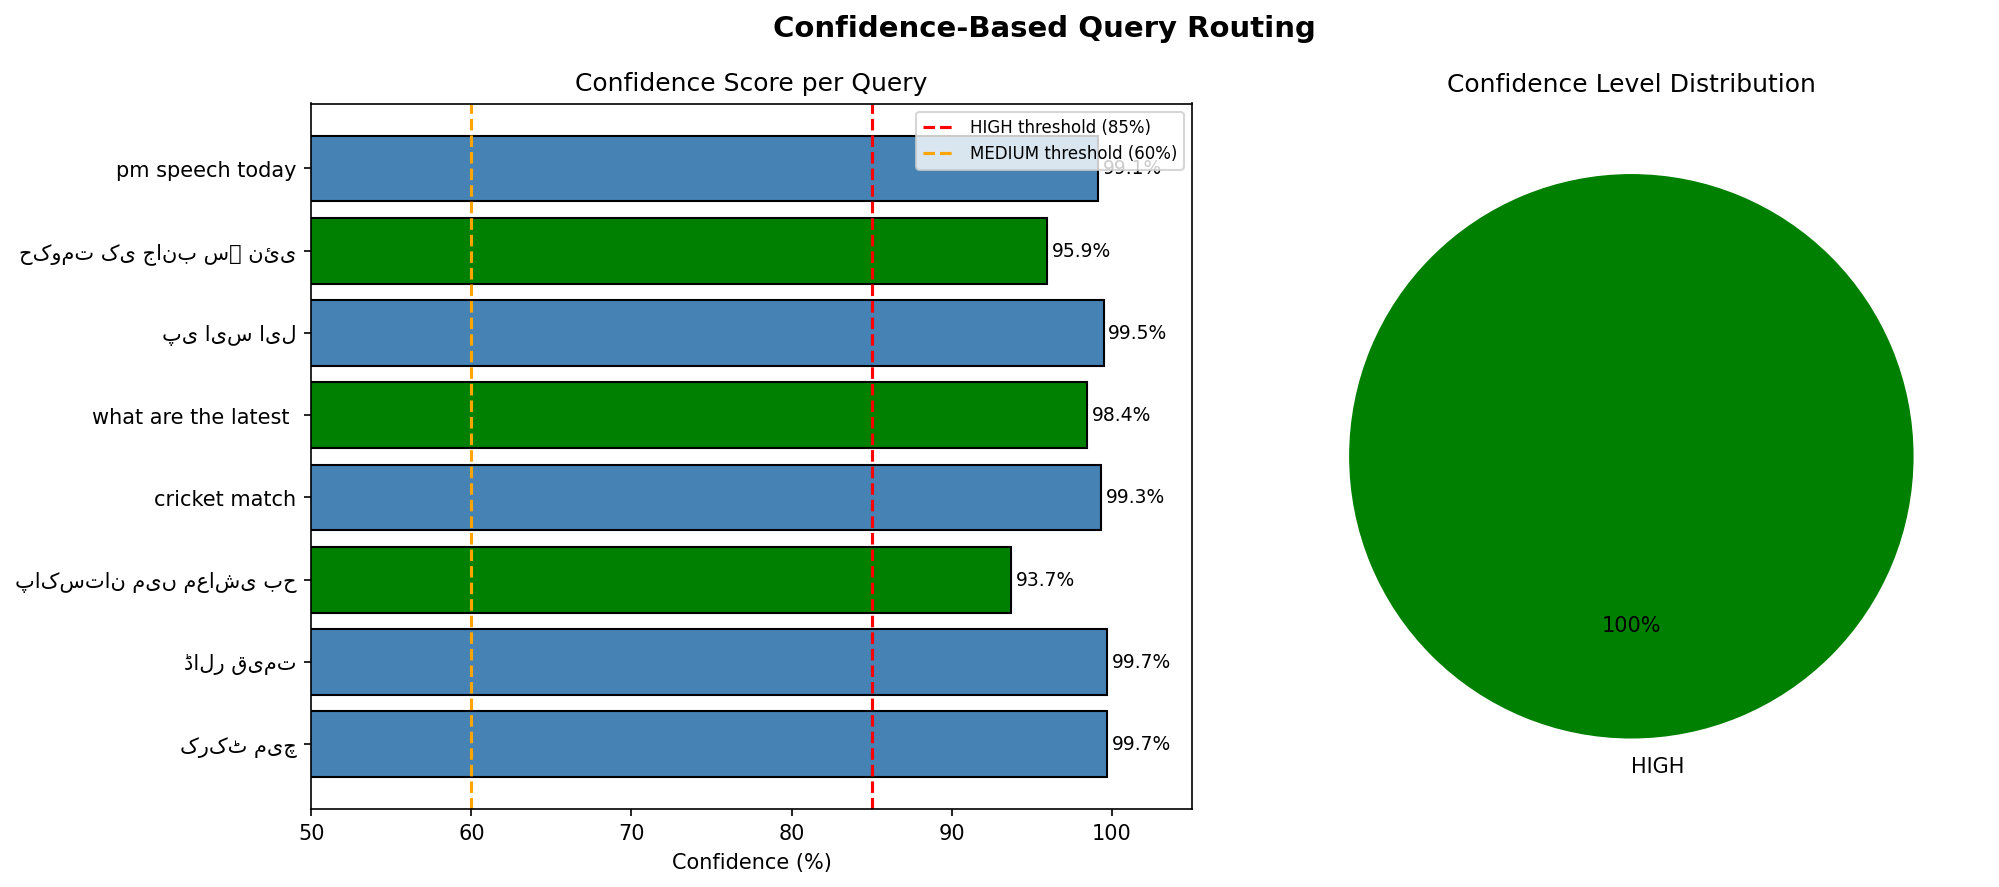
\includegraphics[width=0.95\linewidth]{figures/confidence_routing.png}
\caption{\textbf{Development confidence batch.} All eight queries HIGH. Not the live demo.}
\label{fig:confidence_routing}
\end{figure}

\subsection*{Other robustness plots}
\label{sec:res_robustness}

Figs~\ref{fig:cohens_d}--\ref{fig:robustness_report} are development robustness panels (Cohen's $d$, learning curves, $C$ sweep, a 50-query diagnostic set, ROC AUC $=1.000$ on that layer). Table~\ref{tab:robustness_summary} kept the notebook scorecard. Read it as ``the development task was separable,'' not as frozen trap P@5.

\begin{table}[H]
\centering
\caption{\textbf{Development robustness scorecard (notebook). Not Phase 3B / not H001--H040.}}
\label{tab:robustness_summary}
\small
\begin{tabular}{p{3.4cm}cc}
\toprule
\textbf{Test} & \textbf{Result} & \textbf{Notebook threshold} \\
\midrule
Cohen's $d$ (mean) & 3.581 & $\geq 0.8$ \\
Learning curve val.\ acc. & 100.00\% & $\geq 95\%$ \\
External diagnostic ($n=50$) & 100.00\% & $\geq 95\%$ \\
ROC AUC (dev) & 1.000 & -- \\
\bottomrule
\end{tabular}
\end{table}

\begin{figure}[H]
\centering
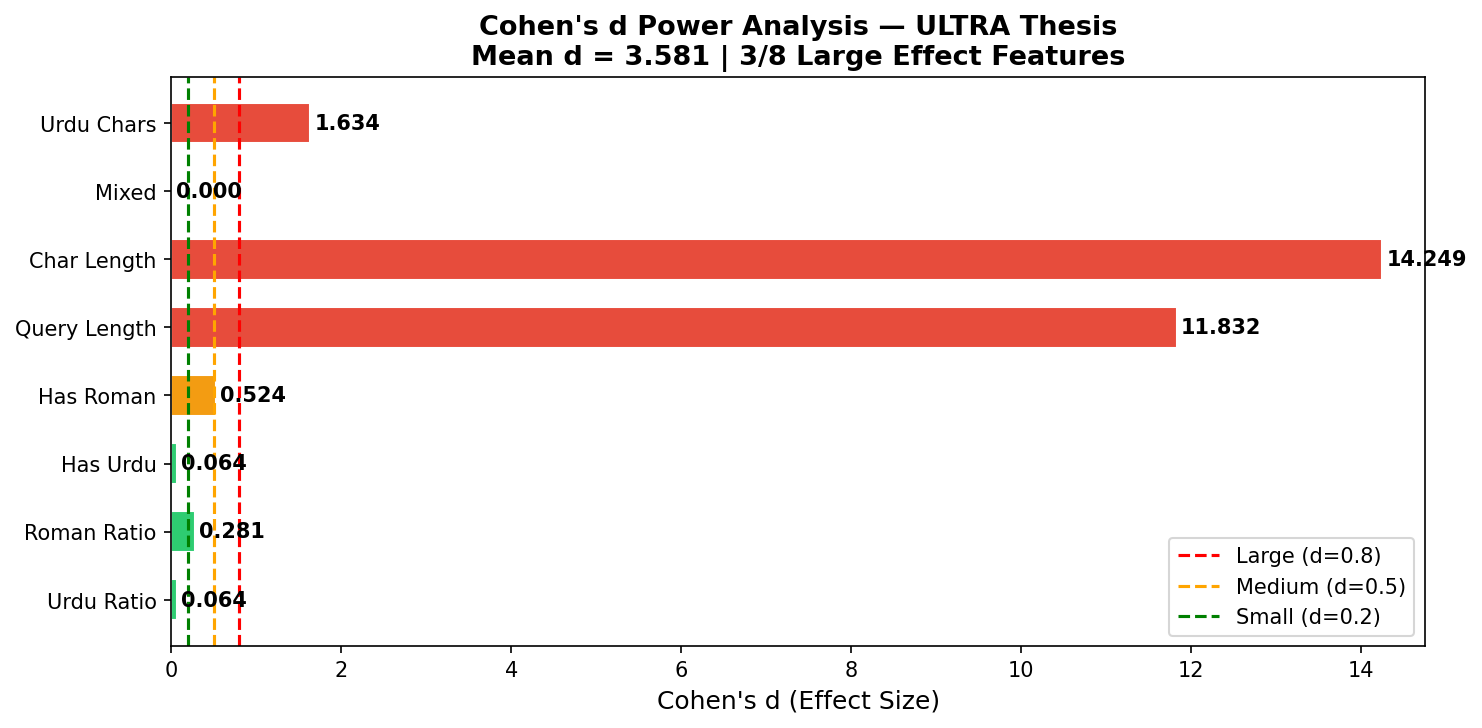
\includegraphics[width=\linewidth]{figures/cohens_d_analysis.png}
\caption{\textbf{Development Cohen's $d$ panel.}}
\label{fig:cohens_d}
\end{figure}

\begin{figure}[H]
\centering
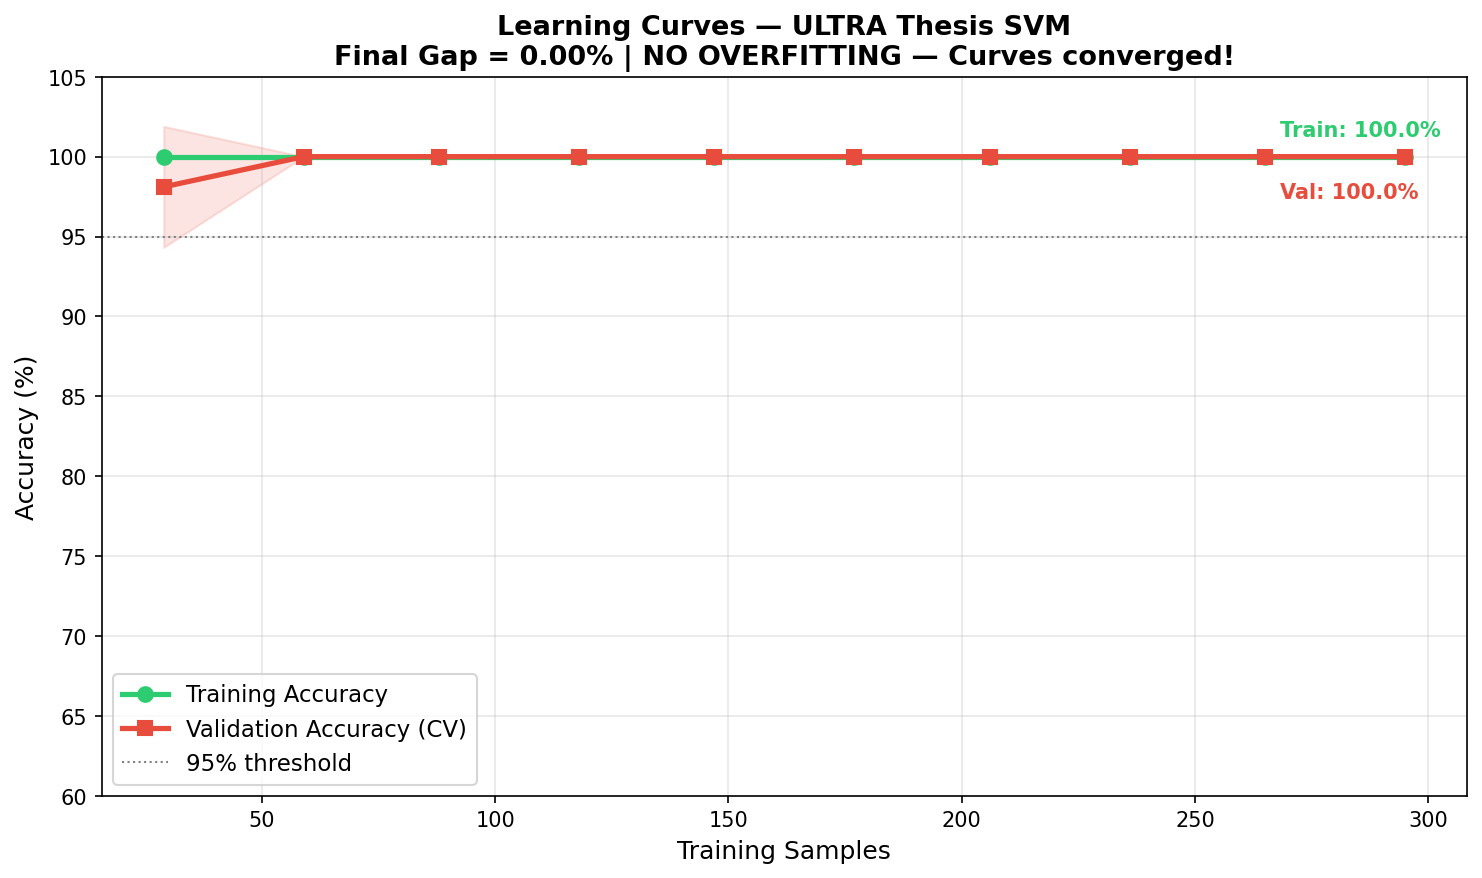
\includegraphics[width=\linewidth]{figures/learning_curves.png}
\caption{\textbf{Development learning curves.}}
\label{fig:learning_curves}
\end{figure}

\begin{figure}[H]
\centering
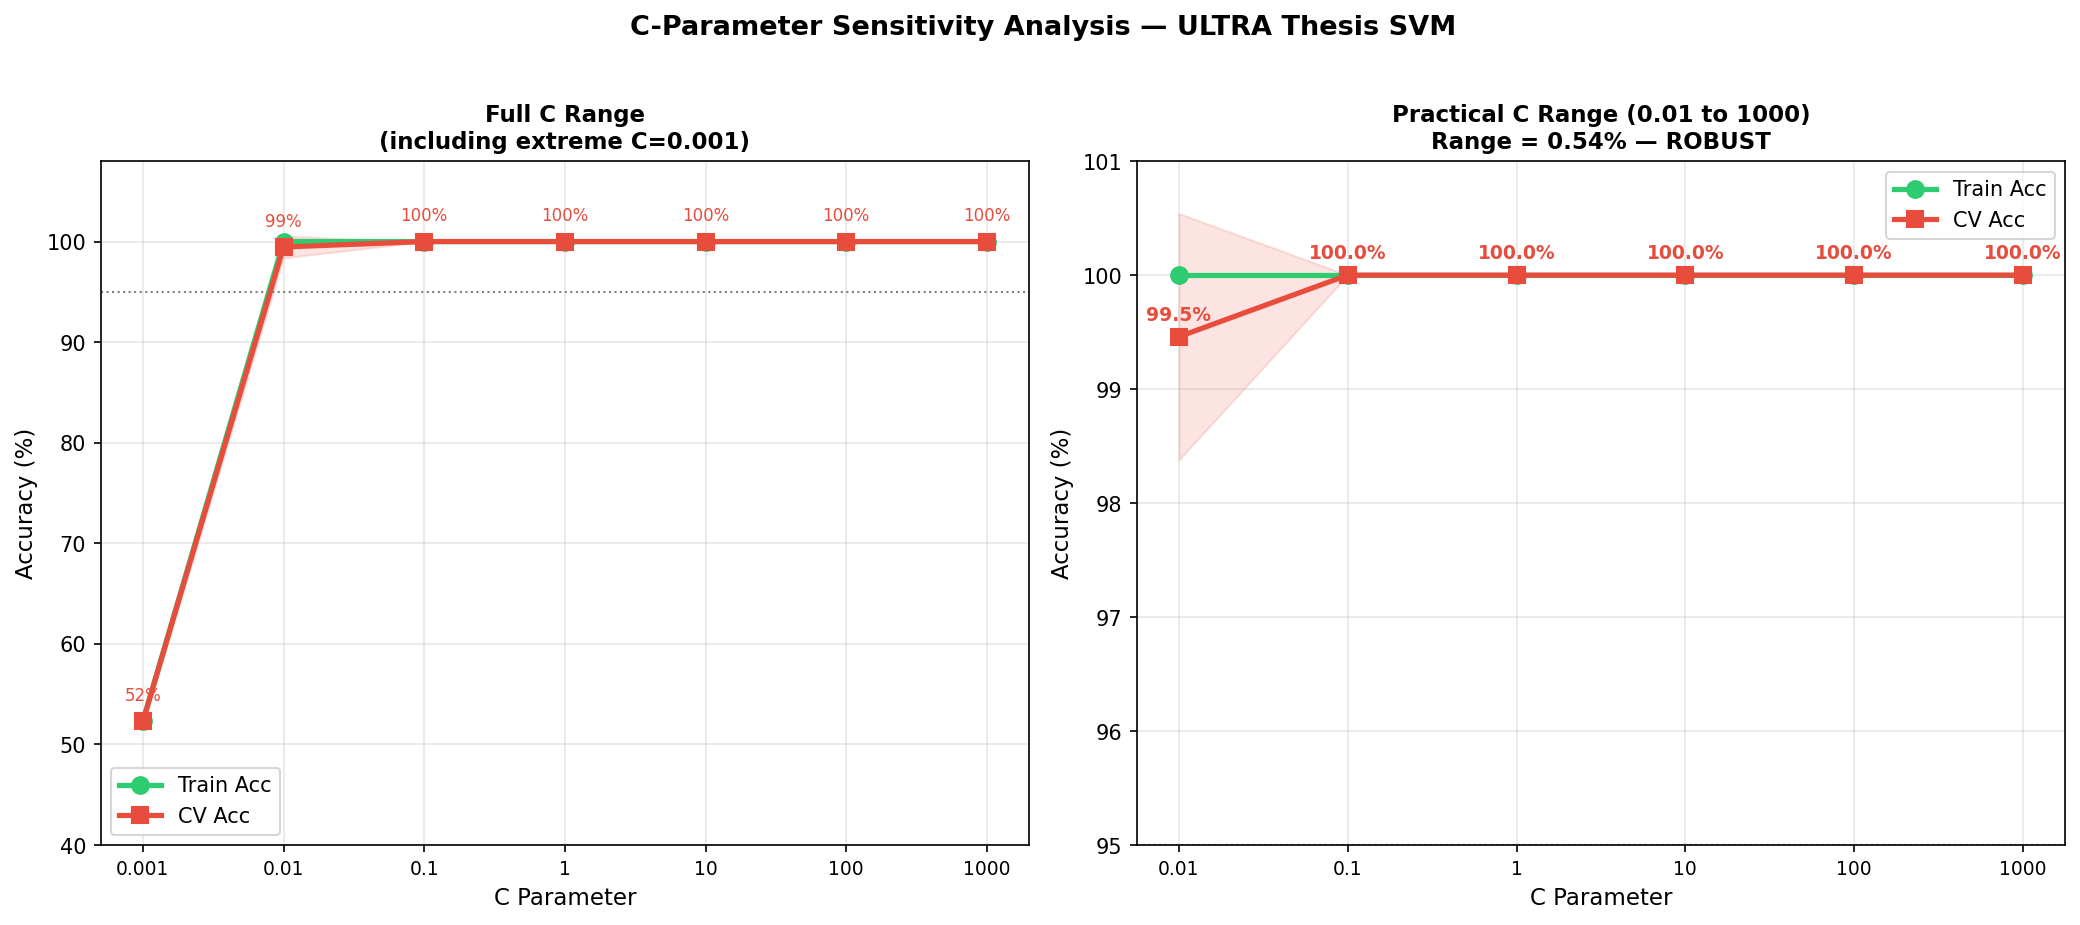
\includegraphics[width=0.95\linewidth]{figures/c_parameter_sensitivity.png}
\caption{\textbf{Development $C$ sweep.}}
\label{fig:c_param}
\end{figure}

\begin{figure}[H]
\centering
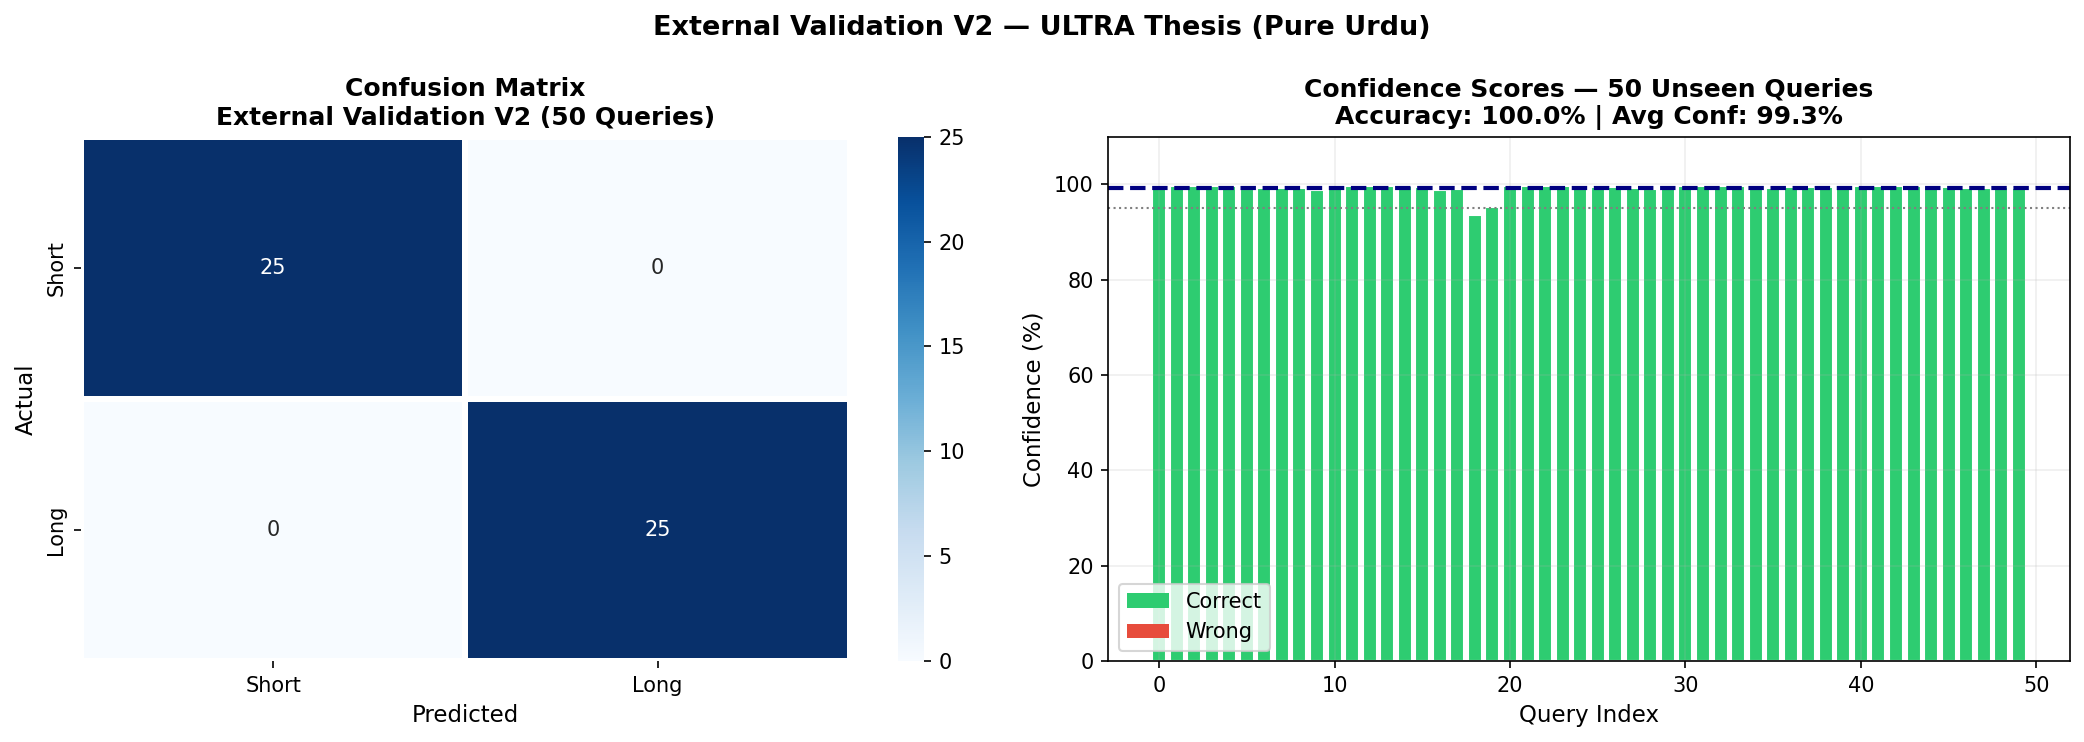
\includegraphics[width=0.95\linewidth]{figures/external_validation.png}
\caption{\textbf{Development diagnostic on 50 native-Urdu queries.} Not the frozen trap sheet.}
\label{fig:external_val}
\end{figure}

\begin{figure}[H]
\centering
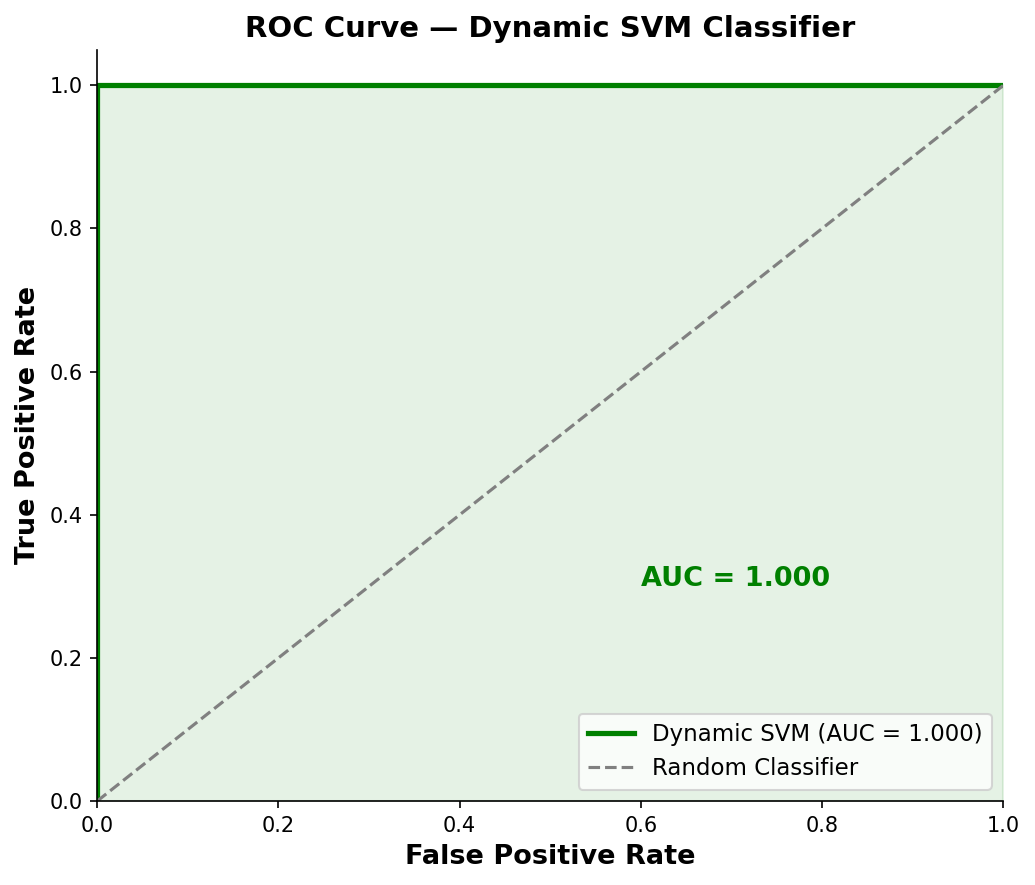
\includegraphics[width=\linewidth]{figures/roc_curve.png}
\caption{\textbf{Development ROC} (AUC $=1.000$ on that layer).}
\label{fig:roc}
\end{figure}

\begin{figure}[H]
\centering
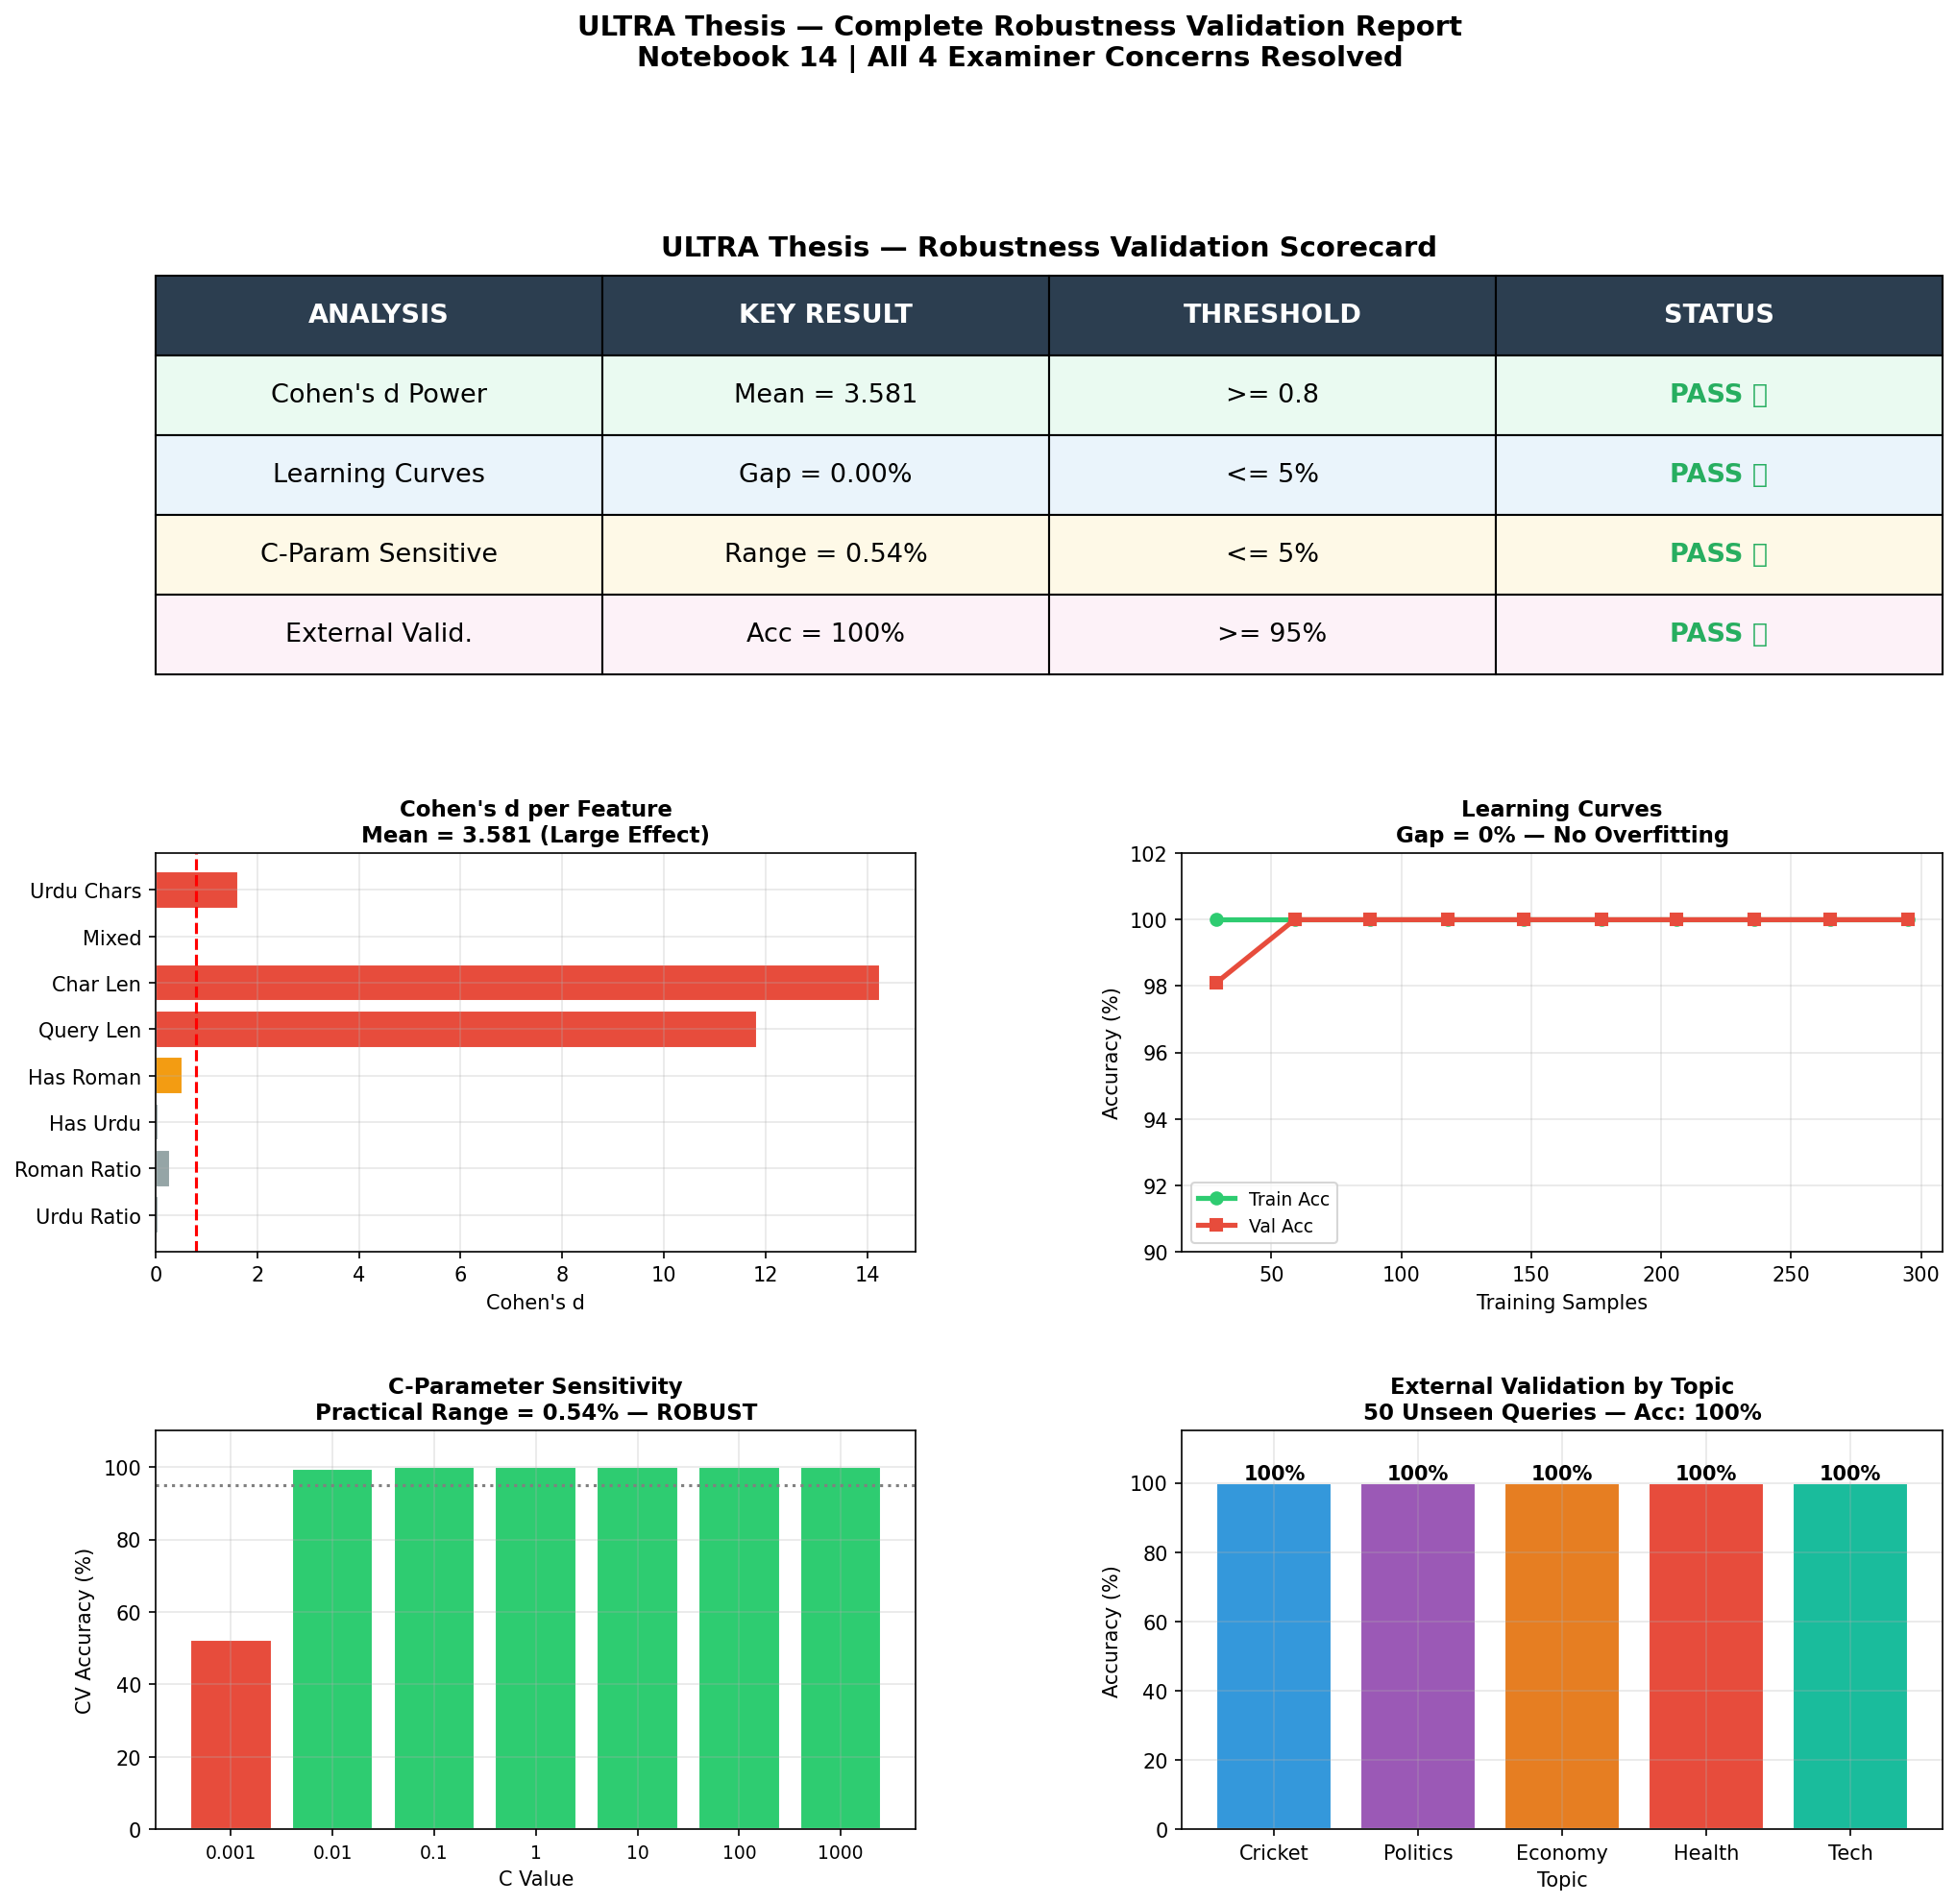
\includegraphics[width=0.95\linewidth]{figures/robustness_final_report.png}
\caption{\textbf{Development robustness collage.}}
\label{fig:robustness_report}
\end{figure}

\subsection*{Discussion}
\label{sec:res_discussion}

There are two readings, and they are not the same paper.

Reading A: 150 characters is the wrong switch. A small SVM, given script and cue features, can beat a word-count rule on queries written to punish that rule. We believe Reading A. The 16--0 McNemar table is hard to argue with if the cue split is printed next to it.

Reading B: therefore the first page of results gets better. We do not have Reading B. Always searching headlines even won nDCG@5. Labels are about need. MiniLM still likes lexical overlap in titles. Medium-confidence mixing can import junk. Forty queries is a small IR test. All of that can be true at once.

English adaptive retrieval usually leads with ranking metrics \cite{arabzadeh2021predicting,jeong2024adaptiverag}. If we had led with development 100\%, the PDF would look cleaner and be worse. PLOS ONE asks whether the study is technically sound, not whether P@5 went up \cite{plosone_criteria}.

% ============================================================
\section*{Conclusion}
\label{sec:conclusion}
% ============================================================

We replaced ULTRA's 150-character switch with a need-based SHORT/LONG label, an eight-feature SVM, two indexes, and a confidence mixer. The SVM is easy to beat word count with when the query contains why/how/fact wording, and it is not easy when those words are absent. Wiring the decision into retrieval did not improve P@5 on 40 frozen traps. nDCG@5 favored headlines for every query. That is the study.

\subsection*{Limitations}
\label{sec:limitations}

News text only. Roman Urdu is a word list, not a trained transliterator. Labels were not a formal double-blind rater study. The deployed twelve-feature pickle is not the frozen V2 scorer. LOW rarely fires on the queries we tried. P@5 cannot see a useful article at rank 8.

\subsection*{Future work}
\label{sec:future_work}

Larger frozen judgment pools. A second human rater. A learned transliterator. Encoders that are not MiniLM. Session context. A live log, not only offline P@5.

\section*{Acknowledgments}

Air University's Department of Creative Technologies supported the MS work behind this manuscript. Funding, data, and author-contribution fields belong in the PLOS submission form, not here.

\nolinenumbers

\bibliography{references}

\end{document}
